\documentclass{book}
\setlength{\parindent}{0cm}
\usepackage[a4paper,margin=2cm]{geometry}

\usepackage[utf8]{inputenc}
\usepackage[french]{babel}
\usepackage{amsmath,amssymb}
\usepackage{stmaryrd}
\usepackage{mathtools} 
\usepackage{extarrows}
\usepackage{oplotsymbl}

\usepackage{graphicx}
\usepackage{psfrag}
\usepackage{caption}
\usepackage{subcaption}
\usepackage{verbatim}
\usepackage{float}

\usepackage{minted}		% Coloration syntaxique
\usepackage[T1]{fontenc}	% Style de ~ incorrect
\usepackage{lmodern}		% Style de ~ incorrect
%\usemintedstyle{upsud}
\newcommand{\inline}[1]{\mintinline[breaklines]{c++}{#1}}
\usepackage{fontspec}
\newfontfamily\dejavusans{DejaVu Sans Mono}[NFSSFamily=DejaVu Sans Mono]

% Meilleures couleurs
\usepackage{xcolor}
\definecolor{red}{RGB}{221,42,43}
\definecolor{green}{RGB}{132,184,24}
\definecolor{blue}{RGB}{0,72,112}
\definecolor{orange}{RGB}{192,128,64}
\definecolor{gray}{RGB}{107,108,110}

\usepackage[onehalfspacing]{setspace}
\setstretch{1.02}

% Solutions encadrées
\usepackage{tikz}
\usepackage[framemethod=tikz]{mdframed}
\newmdenv[
  singleextra={
    \fill[blue] (P) rectangle ([xshift=-15pt]P|-O);
    \node[overlay,anchor=south east,rotate=90,font=\color{white}] at (P) {\sf\textbf{Correction}};
  },
  firstextra={
    \fill[blue] (P) rectangle ([xshift=-15pt]P|-O);
    \node[overlay,anchor=south east,rotate=90,font=\color{white}] at (P) {\sf\textbf{Correction}};
  },
  secondextra={
    \fill[blue] (P) rectangle ([xshift=-15pt]P|-O);
    \node[overlay,anchor=south east,rotate=90,font=\color{white}] at (P) {\sf\textbf{Correction}};
  },
  backgroundcolor=blue!2,
  linecolor=blue,
  skipabove=12pt,
  skipbelow=12pt,
  innertopmargin=0.4em,
  innerbottommargin=0.4em,
  innerrightmargin=2.7em,
  rightmargin=0.7em,
  innerleftmargin=1.7em,
  leftmargin=0.7em,
]{correction}

% Pour cacher/montrer les solutions, décommenter/commenter les 3 lignes ci-dessous
\usepackage{comment}
% \renewenvironment{correction}{}{}
% \excludecomment{correction}

% Fancy chapters
\makeatletter
  \renewcommand{\@chapapp}{TD}
\makeatother

\usepackage{fancyhdr}
\usepackage{fncychap}
  \ChTitleVar{\Huge\bfseries\sffamily\color{blue}}
  \ChNameVar{\raggedleft\fontsize{22}{16}\selectfont\sffamily\color{blue}}
  \ChNumVar{\raggedleft\fontsize{60}{62}\selectfont\sffamily\color{blue}}

% Fancy sections
\usepackage{titlesec}
\titlespacing*{\chapter}{0pt}{-50pt}{40pt}
\titleformat{\section}[block]
  {\Large\bfseries\sffamily\color{blue}}
  {\thesection}
  {1em}
  {}

\newmdenv[nobreak,backgroundcolor=red!20,roundcorner=10pt,linecolor=white]{warning}

\newenvironment{prompt}{\begin{quote}\color{blue!75}\tt\$\,
}{\end{quote}}

\newcommand{\cc}{\mbox{C}}
\newcommand{\cpp}{\mbox{C\vspace{.5em}\protect\raisebox{.2ex}{\footnotesize++~}}}

\def\filename{\emph}


\usepackage{hyperref}

\begin{document}

\setcounter{chapter}{2}

\chapter{Encapsulation, méthodes MCMC et modèle d'Ising}

Le but de ce TD est de comprendre la notion d'encapsulation, de se familiariser avec les mot-clés \inline{public} et \inline{private} et d'introduire la notion de constructeur.\\

Nous allons écrire une classe représentant un réseau 2D, que nous utiliserons pour écrire une simulation Monte-Carlo par chaînes de Markov du modèle d'Ising.

\section{Synchronisation d'attributs}

Imaginons que nous souhaitons modifier la classe \inline{complexe} afin d'y stocker sa représentation polaire (norme, argument) pour, par exemple, éviter de recalculer systématiquement la norme et l'argument à chaque appel des méthodes \inline{norme()} et \inline{argument()}. C'est pertinent si l'accès est beaucoup plus fréquent que la modification.\\

Un problème se pose immédiatement : comment s'assurer que les deux représentations (partie réelle, partie imaginaire) et (norme, argument) restent synchronisées lorsque l'utilisateur modifie, par exemple, la partie réelle ?\\

Il faut que la classe s'occupe elle-même de ses attributs, et empêche l'utilisateur d'y accéder directement. C'est l'encapsulation : les membres deviennent \inline{private}, et leur accès ou modification est permise via des méthodes publiques contrôlées. Une bonne pratique peut être d'appeler un membre privé \inline{type p_membre} (où \inline{type} est le type du membre), et d'appeler les fonctions setter \inline{void set_membre(type valeur)} et les fonctions getter \inline{type membre() const} respectivement. Les fonctions setter et getter (comme leur dénomination l'indique) permettent respectivement de :
\begin{itemize}
\item modifier un attribut de classe \inline{private} (et éventuellement imposer des contraintes, mettre à jour d'autres membres...)
\item obtenir par retour la valeur d'un attribut de classe \inline{private}.
\end{itemize}

Dans la déclaration de la fonction membre getter \inline{type membre() const}, le mot-clé \inline{const} à la fin vient préciser que la méthode ne peut pas modifier l'objet : en effet un getter se contente donc de lire les données de l'objet sans le modifier. Une fonction déclarée \inline{const} ne peut donc pas contenir d'instructions telles que \inline{p_membre = nouvelleValeur}, et ne peut faire appel qu'à des fonctions déclarées \inline{const}. Cela permet, entre autre, au compilateur d'optimiser le code, et à l'utilisateur de manipuler des références constantes d'objet pour éviter des copies inutiles.

\subsection{Encapsulation de la classe \mintinline{c++}{complexe}}

Faire le travail d'encapsulation pour la classe \inline{complexe}. On appellera \inline{double real() const} la fonction permettant d'accéder à la partie réelle du nombre, et \inline{void set_real(double valeur)} la méthode permettant de changer la partie réelle. En ce qui concerne la partie imaginaire, on nommera les méthodes \inline{double imag() const} et \inline{void set_imag(double valeur)}.

Note : le \cpp permet de surcharger les fonctions - deux fonctions peuvent avoir le même nom si leurs arguments sont différents, ou bien si une des fonctions est \inline{const} et l'autre non. Si l'on préfère, on peut donc nommer les setter ainsi : \inline{void real(double valeur)} et \inline{void imag(double valeur)}.\\

Précédemment, on déclarait un nombre complexe de la manière suivante : \inline{complexe nombre;}. En l'absence de constructeur, ni la partie réelle ni la partie imaginaire ne sont initialisées, et peuvent donc avoir des valeurs arbitraires. Écrivez donc trois constructeurs : le constructeur par défaut ($0+0\mathrm{i}$), le deuxièle prenant un simple \inline{double} (le complexe aura alors une partie imaginaire nulle), et le dernier prenant une partie réelle et une partie imagainaire. Supprimer l'éventuelle méthode d'initialisation provenant du TD précedent.\\

Comme toujours, tester votre classe et ses méthodes.

\subsection{Modification de la logique interne}

Maintenant que l'encapsulation est faite, on peut se permettre de modifier le fonctionnement interne de la classe \emph{sans changer quoi que ce soit pour l'utilisateur}, ie. sans modifier le programme de test. C'est un avantage majeur de l'encapsulation.\\

Ajouter des attributs privés stockant la norme et l'argument comme présenté en introduction. Modifier les setters et les constructeurs pour garder sychronisé ces nouveaux attributs polaires avec les attributs carthésiens, et vice-versa, lorsque des modifications sont effectuées. On rajoutera enfin un setter \inline{void set_polar(double r, double theta)}.\\

En résumé on veut que :
\begin{itemize}
  \item à chaque fois que la partie réelle ou imaginaire est modifiée, les attributs stockant la norme et l'argument soient mis à jour aussi
  \item à chaque fois que la norme ou l'argument est modifiée, les attributs stockant les parties réelles et imaginaires soient mis à jour aussi
\end{itemize}
pour que nos 4 attributs soient toujours synchronisés.\\

Pour éviter de dupliquer le code, on pourra éventuellement créer des méthodes privées \inline{void sync_carth_to_polar()} et \inline{void sync_polar_to_carth()}.\\

Pour ne pas passer trop de temps sur ce TD, on pourra supprimer les opérateurs surchargés (en particulier les opérateurs modifiant l'objet : \inline{+=}, \inline{*=}...).

On gardera toutefois l'opérateur de multiplication entre deux complexes, et on simplifiera son implémentation à l'aide des coordonnées polaires pré-calculées : $(r\mathrm{e}^{\mathrm{i}\theta})\cdot(r'\mathrm{e}^{\mathrm{i}\theta'})=r\,r'\mathrm{e}^{\mathrm{i}(\theta+\theta')}$.
Enfin, proposer un opérateur de division entre un scalaire et un complexe, \inline{complexe operator/ (double left, complexe right)} utilisant les coordonnées polaires pré-calculées.\\

Testez votre classe et ses fonctionnalités.

\begin{correction}
La déclaration de la classe \inline{complexe} devient donc
\begin{minted}[breaklines]{c++}
class complexe {
private:
  double p_real, p_imag, p_mag, p_arg;

  void sync_carth_to_polar ();
  void sync_polar_to_carth ();

public:
  complexe ();
  complexe (double r);
  complexe (double r, double i);

  double real () const { return p_real; }
  void set_real (double re);

  double imag () const { return p_imag; }
  void set_imag (double im);

  void set_polar (double r, double theta);

  double norme () const { return p_mag; }
  double argument () const { return p_arg; }

  complexe operator* (complexe right);
};
\end{minted}

La définition des getters est maintenant triviale grâce au pré-calcul des coordonnées dans les deux systèmes. Ils sont tellement simples que nous nous sommes permis de les définir directement dans le header, ce qui est tout à fait autorisé.\\

Une fois que \inline{sync_carth_to_polar()} et \inline{sync_polar_to_carth()} ont été écrites, la définition des autres méthodes est simple :

\begin{minted}[breaklines]{c++}
/* Mise à jour des coordonnées polaires <-> carthésiennes */

void complexe::sync_carth_to_polar () {
  p_mag = sqrt(p_real*p_real + p_imag*p_imag);
  p_arg = atan2(p_imag, p_real);
}

void complexe::sync_polar_to_carth () {
  p_real = p_mag * cos(p_arg);
  p_imag = p_mag * sin(p_arg);
}

/* Setters */

void complexe::set_real (double re) {
  // on change la valeur de la partie réelle
  p_real = re;
  // donc on met à jour la norme et l'argument
  sync_carth_to_polar();
}

void complexe::set_imag (double im) {
  // on change la valeur de la partie imaginaire
  p_imag = im;
  // donc on met à jour la norme et l'argument
  sync_carth_to_polar();
}

void complexe::set_polar (double r, double theta); {
  // on change les coordonnées polaires
  p_mag = r;
  p_arg = theta;
  // donc on met à jour de la partie réelle et imaginaire
  sync_polar_to_carth();
}
\end{minted}

Quand aux constructeurs, leur implémentation peut être
\begin{minted}[breaklines]{c++}
complexe::complexe (double r) {
  p_real = p_imag = p_mag = p_arg = 0;
}

complexe::complexe (double r) {
  p_real = r;
  p_imag = 0;
  p_mag = r;
  p_arg = 0;
}

complexe::complexe (double r, double i) {
  p_real = r;
  p_imag = i;
  sync_carth_to_polar();
}
\end{minted}

Toutefois, c'est une bonne habitude d'utiliser les listes d'initialisation :

\begin{minted}[breaklines]{c++}
complexe::complexe () : complexe(0) {}

complexe::complexe (double r) :
  p_real(r), p_imag(0), p_mag(r), p_arg(0)
{}

complexe::complexe (double r, double i) :
  p_real(r), p_imag(i)
{
  sync_carth_to_polar();
}
\end{minted}

Notons que pour le constructeur par défaut, nous avons simplement ré-utilisé le deuxième constructeur.\\

Pour la multiplication de deux complexes, on a choisi ici de définir un opérateur membre de la classe. Son implémentation est très simple en coordonnées polaires :
\begin{minted}[breaklines]{c++}
complexe complexe::operator* (complexe right) {
  complexe res;
  res.p_mag = p_mag * right.p_mag;
  res.p_arg = p_arg + right.p_arg;
  // on n'oublie pas de synchroniser les coordonnées carthésiennes
  res.sync_polar_to_carth();
  return r;
}
\end{minted}

Alternativement, on aurait pu utiliser \inline{res.set_polar()}, et la synchronisation aurait été automatique.\\

L'opérateur de division d'un scalaire par un complexe doit être défini à l'extérieur de la classe, et n'a donc pas accès aux attributs directement. Toutefois, son implémentation est simple et efficace grâce aux méthodes définies précédemment :

\begin{minted}[breaklines]{c++}
complexe operator/ (double left, complexe right) {
  // on a pris `right' par copie, on peut donc le modifier
  // le calcul de l'inverse de right est très simple en coordonnées polaires :
  right.set_polar(
    left / right.norme(), // norme
    -right.arg()          // argument
  );
  return right;
}
\end{minted}

Enfin, l'opérateur de flux (ainsi que la fonction non-membre \inline{exponentielle}) se voient légèrement modifiés, car on a changé la façon dont on accède aux parties réelles et imaginaires :
\begin{minted}[breaklines]{c++}
ostream& operator<< (ostream& out, const complexe& z) {
  if (z.imag() >= 0) {
    out << z.real() << "+" << z.imag() << "i";
  } else {
    out << z.real() << "-" << -z.imag() << "i";
  }
  return out;
}
\end{minted}

Notons enfin que les attributs contenus dans notre classe \inline{complexe} ne nécessitent aucune action particulière lors de leur création ou destruction. De plus, notre classe ne gère aucune ressource, et les attributs peuvent être simplement copiés pour copier un nombre complexe. Il n'est donc pas nécessaire de définir le constructeur par copie, le destructeur ou l'opérateur d'affectation.
\end{correction}

\section{Un réseau 2D}

Nous voulons créer une classe \inline{Réseau} matéralisant un réseau en deux dimensions, avec des conditions périodiques aux limites, c'est-à-dire un ensemble périodique de sites dans un espace sans bords. L'objectif va être d'écrire une interface suffisemment générique pour pouvoir simuler, par exemple, le modèle d'Ising, que ça soit sur un réseau carré, triangulaire, hexagonal...\\

Le hamiltonien du modèle d'Ising étant local (voir la section suivante), la seule chose qui nous intéresse réellement est d'accéder aux \emph{voisins} d'un site, sans se soucier de ses coordonnées précises. C'est en cela que la classe pour un réseau carré va différer d'une simple matrice. Il s'agit, en quelque sorte, d'invisibiliser la structure précise du réseau à l'algorithme l'utilisant.\\

\subsection{Écriture de la classe \inline{Réseau}}
\emph{Il est conseillé de lire l'énoncé de toute cette section en entier avant de commencer l'écriture du code. Cette classe peut sembler intimidante à écrire, mais en s'y prennant bien, \filename{reseau.h} et \filename{reseau.cpp} peuvent avoir une taille de l'ordre de 60 lignes de code seulement chacun, commentaires inclus. Une heure devrait suffire.}\\

Comme dans l'exemple de la classe \inline{Matrice} présenté en cours, nous allons "aplatir" la matrice en un tableau 1D, car c'est plus performant que de faire des tableaux de tableaux, et car cela se généralise mieux à un réseau quelconque. Une position $(x,y)$ sera alors encodée par l'indice $i = x + n_x \times y$ (ou $i' = n_y \times x + y$ si l'on préfère) :
\begin{equation*}
[a_{x y}]_{x, y} = \left[\begin{array}{cc}
     a_{0 0} & a_{0 1}\\
     a_{1 0} & a_{1 1}\\
     a_{2 0} & a_{2 1}
   \end{array}\right] \quad \longrightarrow \quad [a_i]_i = \left[a_{0 0}, a_{0 1},
   a_{1 0}, a_{1 1}, a_{2 0}, a_{2 1}\right] 
\end{equation*}
Pour des raisons de performance, il est parfois plus utile de travailler avec $(x,y)$ ou avec $i$. Comme le simulation du modèle d'Ising nécessite les deux, nous allons conserver ces deux types d'indice dans un type commun \inline{Site} :
\begin{minted}[breaklines]{c++}
class Site {
  int _index;
  int _x;
  int _y;
};
\end{minted}
Ceci est pour un réseau carré, et les plus courageux feront le reste du TD avec un réseau hexagonal (ou plus exactement \emph{en nid d'abeille}) pour pimenter l'exercice\footnote{Le réseau hexagonal est plus compliqué à implémenter car bipartite (ce n'est pas un réseau de Bravais). Dans ce réseau, chaque site est relié à 3 voisins contrairement à 4 pour un réseau carré ou à 6 pour un réseau triangulaire. Une façon de faire est de stocker les deux réseaux de Bravais de façon interlacée, et de spécifier, en plus de \inline{x} et \inline{y}, sur quel sous-réseau de Bravais le site est situé, et donc introduire une 3è coordonnée (\inline{a} par exemple, qui vaudra \inline{true} ou \inline{false}).}. Pour un niveau de difficulté intermédiaire, on pourra tenter un réseau triangulaire\footnote{Qui, lui, est un réseau de Bravais et peut être représenté comme une matrice, comme le réseau carré. Dans le réseau triangulaire, chaque site interragit avec 6 sites voisins.}.

Ici, nous utilisons la classe \inline{Site} comme un simple tuple, et nous choisissons de mettre toute la logique de traduction entre $(x,y)$ et $i$ dans la classe \inline{Réseau}.\footnote{On pourrait faire l'inverse, et mettre des méthodes de synchronisation comme pour la classe \inline{complexe} ci-dessus. Mais en terme de performance, il est plus simple de faire comme ci-dessous.}

Comme \inline{_index}, \inline{_x} et \inline{_y} seront gérés et synchronisés par la classe \inline{Réseau} uniquement, et que l'utilisateur n'a pas à trifouiller ces données internes, nous allons les déclarer \inline{private}. On parle de type \emph{opaque}. En contrepartie, il faudra autoriser la classe \inline{Réseau} à y accéder. Une solution adaptée est d'utiliser une notion qui n'a pas été vue en cours : les classes et fonctions amies. Pour faire court, si la classe \inline{Site} déclare \inline{Réseau} comme classe amie, ses attributs privés seront accessibles dans les méthodes de \inline{Réseau}. Il faut utiliser le mot-clé \inline{friend} pour cela :
\begin{minted}[breaklines]{c++}
class Site {
private:
  int _index;
  int _x;
  int _y;

  friend class Réseau;

  Site (int i, int x, int y) : _index(i), _x(x), _y(y) {}
  Site () = default;

public:
  int x () const { return _x; }
  int y () const { return _y; }
};
\end{minted}
Nous avons au passage ajouté deux constructeurs, ce qui est nécessaire dès lors que l'on a des attributs privés, ainsi que deux accesseurs \inline{x()} et \inline{y()}. Aucune autre méthode que ces constructeurs et accesseurs n'est nécessaires. Le type \inline{Site} est tellement simple qu'il n'y a pas besoin de créer une paire \filename{.h}/\filename{.cpp} associée. N'hésitez pas à ajouter un opérateur de flux pour afficher les coordonnées d'un site\footnote{Par exemple: \inline{std::ostream& operator<< (std::ostream& out, const Site& s) { out << "(" << s.x() << "," << s.y() << ")"; return out; }}}.\\

Nous allons maitenant écrire une classe \inline{Réseau} en s'inspirant de la classe \inline{Matrice} vue en cours pour le stockage de données (allocation dynamique au lieu d'utiliser \inline{std::vector})\footnote{Bien sûr, dans la vraie vie, on ne s'embête pas à faire cette allocation manuelle, on utilisera les types automatiques déjà présent dans la bibliothèque standard.}. Notre matrice sera de type \inline{int8_t}, qui est le plus petit entier signé possible\footnote{C'est en fait équivalent à un \inline{char}. Si vous essayez d'affichez la valeur de votre pointeur vers la zone mémoire stockée avec \inline{std::cout}, vous passez donc un \inline{char*}, qui sera interprété comme une chaine de caractère... ce qui n'est pas ce que l'on veut. Il faut alors convertir en, par exemple, un \inline{void*}. On écrira alors \inline{cout << (void*)data;}. De même, si vous voulez afficher directement un \inline{int8_t} avec \inline{std::cout}, ça ne va pas fonctionner car il va l'interpréter comme un caractère et non un entier. On écrira alors \inline{cout << (int)data[i];}. Pour utiliser les types comme \inline{intN_t}, il vous faudra sans doute inclure \inline{stdint.h}.}. Les tailles $n_x$ et $n_y$ seront stockées sous forme de constantes. Écrivez un constructeur \inline{Réseau (int nx, int ny, int8_t valeur_def)}, ainsi qu'un destructeur et un constructeur par copie. Bien sûr, testez votre code en créant une matrice, puis en la copiant. On pourra rajouter temporairement un affichage de l'adresse de l'objet courant ainsi que l'adresse de la zone mémoire allouée, pour être certain que l'on fait correctement les choses.\\

Une fois cette base écrite, créez deux méthodes dans la classe \inline{Réseau} pour générer un objet de type \inline{Site} :
\begin{itemize}
  \item Une méthode privée "\inline{Site site_index (int index) const;}" prenant en argument l'indice $i$ et déduisant $x$ et $y$ (privée car l'utilisateur de la classe n'a que faire de cet indiçage interne, et constante car il n'y a pas modification de l'objet).
  \item Une méthode publique "\inline{Site site_xy (int x, int y) const;}" prenant en argument $x$ et $y$ et déduisant $i$. Les conditions limites périodiques seront implémentés ici, et on ramènera systématiquement $x$ et $y$ dans $\llbracket 0,n_x\!-\!1 \rrbracket$ et $\llbracket 0,n_y\!-\!1\rrbracket$ respectivement\footnote{Attention, le modulo \texttt{\%n} appliqué sur un entier signé ramène l'entier dans $\rrbracket-n,n\llbracket$, au plus proche de zéro, ce qui n'est pas pratique pour nous. Un façon perfomante de faire est d'ajouter $n$ au résultat du modulo si celui-ci est négatif.}.
\end{itemize}
On écrira aussi une méthode \inline{Site site_aleatoire () const;} renvoyant un site aléatoire du réseau.\\

Ensuite, ayant un "\inline{Site s;}" il nous faut une méthode pour accéder à la valeur du site \inline{s}. Pour cela, on définiera \inline{int8_t operator[] (Site) const;} et \inline{int8_t& operator[] (Site);} pour respectivement lire et modifier un site. Exemple d'utilisation :
\begin{minted}[fontsize=\footnotesize]{c++}
Site s = mon_reseau.site_xy(7,15);
cout << mon_reseau[s] << endl; // lecture de la valeur du site (7,15)
mon_reseau[s] = 4; // modification de la valeur du site (7,15), rendu possible car une référence int8_t& est renvoyée
\end{minted}
Optionnellement, on pourra déclarer \inline{int8_t& operator[] (int x, int y);} pour que l'utilisateur puisse accéder directement à un site $(x,y)$ sans avoir à écrire "\inline{mon_reseau[mon_reseau.site_xy(x,y)]}". Attention, l'opérateur \inline{[]} à plusieurs arguments n'existe que depuis le C++23, et il faut donc un compilateur suffisemment récent\footnote{GCC 12 ou clang 15, cf. \url{https://en.cppreference.com/w/cpp/compiler_support/23}. Peut nécessiter l'option de compilation \texttt{-std=c++2b} ou \texttt{-std=c++23}.}.\\

Enfin, écrire une méthode \inline{std::array<Site,4> voisins (Site s) const;} qui renvoit les 4 voisins d'un site \inline{s} (ou les 3 voisins pour un réseau hexagonal, ou les 6 voisins pour un réseau triangulaire). On notera l'utilisation de \inline{std::array<Type,N>}\footnote{Présent dans le header \texttt{<array>}}, qui n'est rien d'autre qu'un tableau de taille fixe \inline{N} glorifié, mais plus pratique car permettant, par exemple, d'utiliser les boucles "for in" et de connaître sa taille avec \inline{.size()}. Il peut être initialisé ainsi : \inline{std::array<int,3> tab = { 42, 41, 40 };}. Bien sûr, aidez vous des méthodes déclarées précédemment. Testez cette méthode en demandant les voisins d'un site situé au milieu, ainsi que les voisins d'un site suité au bord du réseau.\\

\begin{correction}
\subsubsection*{Déclaration : fichier \filename{reseau\_carre.h}}

\begin{minted}[fontsize=\footnotesize]{c++}
#include <array>
#include <functional>

class Réseau {
public:

  // Type opaque stockant les coordonnées pré-calculées d'un site
  class Site {
  private:
    int _index;
    int _x;
    int _y;

    Site (int i, int x, int y) : _index(i), _x(x), _y(y) {}
    Site () = default;
    friend class Réseau;

  public:
    int x () const { return _x; }
    int y () const { return _y; }
  };

  // Taille de la matrice de site
  const int nx;
  const int ny;

private:

  // Zone mémoire stockant la matrice repliée
  int8_t* data;
  // Nombre total de sites (0 <= _index < ntot)
  const int ntot;

  // Revoie l'objet Site correspondant à l'indice `index` de la matrice repliée
  Site site_index (int index) const;

public:

  // Revoie l'objet Site correspondant au site de coordonnées (x,y),
  //  en tenant compte des conditions périodiques aux limites
  Site site_xy (int x, int y) const;
  // Revoie l'objet Site correspondant à un site choisi aléatoirement
  Site site_aleatoire () const;

  // Accès à la valeur d'un site
  int8_t operator[] (Site) const; // Accès par valeur sans modification possible
  int8_t& operator[] (Site); // Accès par référence, avec modification possible

  // Lite des sites directement voisins d'un site `s`
  std::array<Site,4> voisins (Site s) const;

  // Construction et destruction
  Réseau (int nx, int ny);
  Réseau (int nx, int ny, int8_t valeur_def);
  Réseau (const Réseau&) = delete;
  ~Réseau ();
};

// Pour éviter d'avoir à tapper `Réseau::Site` à chaque fois
using Site = Réseau::Site;
\end{minted}

Notons que contrairement à ce que l'énnoncé demande, nous n'avons pas implémenté le constructeur par copie, et nous avons donc explicitement désactivé la copie en le déclarant \inline{delete}. Si nous voulons l'implémenter tout de même, il suffit de reprendre celui présenté en cours.

\subsubsection*{Déclaration : fichier \filename{reseau\_carre.cpp}}

\begin{minted}[fontsize=\footnotesize]{c++}
#include "reseau_carre.h"

/* Construction et destruction */

Réseau::Réseau (int nx, int ny) : nx(nx), ny(ny), ntot(nx*ny), data(nullptr) {
  data = new int8_t[nx*ny];
  // note : il est nécessaire d'utiliser une initializer list ici, car nx, ny et ntot sont constants
}

Réseau::Réseau (int nx, int ny, int8_t valeur_def) : Réseau(nx,ny) {
  // ici, le constructeur ci-dessus et appelé par ce constructeur
  for (int i = 0; i < ntot; i++)
    data[i] = valeur_def;
}

Réseau::~Réseau () {
  delete[] data;
}

/* Indiçage des site */

Réseau::Site Réseau::site_index (int index) const {
  // index replié -> (x,y)
  int x = index % nx;
  int y = index / nx;
  return Site(index, x, y);
}

Réseau::Site Réseau::site_xy (int x, int y) const {
  // (x,y) quelconque -> (x,y) replié -> indice replié
  x = x % nx;
  if (x < 0) x += nx;
  y = y % ny;
  if (y < 0) y += ny;
  int index = x + nx * y;
  return Site(index, x, y);
}

#include <random>
std::mt19937 rng_reseau;  // déclaration d'un générateur en tant que variable global (discutable)

Site Réseau::site_aleatoire () const {
  return site_index( rng_reseau() % ntot );
}

/* Accès à la valeur d'un site */

int8_t Réseau::operator[] (Site s) const {
  return data[s._index];
}

int8_t& Réseau::operator[] (Site s) {
  return data[s._index];
}

/* Voisinage d'un site */

std::array<Site,4> Réseau::voisins (Site s) const {
  return {
    site_xy( s._x+1, s._y   ),
    site_xy( s._x,   s._y-1 ),
    site_xy( s._x-1, s._y   ),
    site_xy( s._x,   s._y+1 ),
  };
}
\end{minted}

\subsubsection*{Réseau hexagonal}

La solution est fournie dans les fichiers \filename{TD3/reseau\_hexa.h} et \filename{TD3/reseau\_hexa.cpp}.

\subsubsection*{Itérateurs}

Notons que dans les classes \filename{reseau\_carré.h}:\inline{Réseau} et \filename{reseau\_hexa.h}:\inline{Réseau} des fichiers de correction, on s'est permis de rajouter un élément permettant de passer d'un type de réseau à l'autre sans aucune modification du reste du code : un itérateur sur les sites du réseau. Il est en effet nécessaire de parcourir l'ensemble du réseau parfois (par exemple pour l'initialisation ou le calcul des observables dans la suite du TD). Un parcours utilisant les coordonnées $(x,y)$ dépendrait nécessairement du type du réseau. Pour s'abstraire des coordonnées, on laisse la classe faire le parcours elle-même. L'utilisateur utilise alors l'itérateur et son \inline{operator++} pour avancer d'un site. Cela permet d'écrire des range-based loop, comme ceci :
\begin{minted}[]{c++}
for (Site i : S) {
  faire_quelque_chose_avec S[i];
}
\end{minted}
ce qui a aussi l'avantage d'être bien plus concis. Mais la notion d'itérateurs sort un peu du cadre de ce cours, et il n'est pas du tout nécessaire de la maîtriser.

\end{correction}

\subsection{Affichage}

Nous voulons bien sûr pouvoir afficher notre système, de préférence en temps réel, pour voir les différentes configurations du modèle d'Ising évoluer. La façon la plus simple est d'afficher le réseau dans le terminal sous forme d'une matrice de caractères. Mais on peut faire bien mieux : afficher graphiquement le système dans une fenêtre dédiée. C'est néamoins bien plus compliqué, car il faut installer et faire appel à une bibliothèque externe. Nous faisons ici le choix d'utiliser la SFML pour cette tâche.

\subsubsection{Affichage textuel (réseau carré uniquement)}

Ajouter une méthode \inline{void affiche_console () const;} affichant dans le terminal l'état du système. Dans le but d'utiliser notre classe pour le modèle d'Ising, où les sites du réseau peuvent valoir $\pm 1$, on affichera tout valeur positive par un carré vide/blanc (\mintinline[fontfamily=DejaVu Sans Mono]{text}{□}), tout valeur négative par un carré plein/noir (\mintinline[fontfamily=DejaVu Sans Mono]{text}{■}), et une valeur nulle par un espace. L'affichage d'un système de $20\times 20$ ressemblera alors à ceci :

\begin{minted}[fontsize=\footnotesize,fontfamily=DejaVu Sans Mono,baselinestretch=0.5,samepage]{text}
■□□□□□■■■■■■■■■■■■■□
□□□■□■■■■■■■■■■□■■■□
■□□□□■■■■■□□□■■■□□□□
□□□□□■■■■□□□□□□□□□□□
□□□□□□■□□□□□□□□□□□□□
□□□□□□□□□□■□□□□□■■■□
□□□□□□□□□□■□□□□□■■■□
□□□□□□□□□□□□□□□□□■■□
□□□□■□□□□□□□□□□□□□□□
■□□□□■□□□■■■□□□□□□□□
■□□□□□□□■■■■□□□□□□□□
■□□□□□□□■■■■■■□□□□□□
■□□□□■□■■■■■■■□□□□■□
□□□□□■□□■■■■■■□□□□□■
■■■□□□□□■■■■■□■□□□□□
■■■■■■□■■■■■■□■■□□□□
■■■■■■■■■■■■■■■■■■■■
■■■■■■■■■■■■■■■■■■□■
■■■■■■■■■■■■■■■■■■□□
□□□□□■■■■■■■■■■■■■■■
\end{minted}

\begin{correction}
On déclare la méthode \inline{void affiche_console () const;} comme \inline{public} dans la déclaration de la classe, puis on la définie dans \filename{reseau.cpp}. Voici une implémentation possible :
\begin{minted}[fontsize=\footnotesize,fontfamily=DejaVu Sans Mono]{c++}
#include <iostream>

void Réseau::affiche_console () const {
  for (int y = 0; y < ny; y++) {
    for (int x = 0; x < nx; x++) {
      int8_t v = data[ site_xy(x,y)._index ];
      if (v < 0)
        std::cout << "■";
      else if (v > 0)
        std::cout << "□";
      else
        std::cout << " ";
    }
    std::cout << std::endl;
  }
}
\end{minted}
\end{correction}

\subsubsection{Affichage graphique avec la SFML}

Cette partie est réservée aux plus rapides. Les autres pourrons toujours y revenir, notamment pour l'affichage graphique pour les projets. La première étape est de suivre le tutoriel SFML (\filename{Tuto SFML.pdf}).\\ 

Ajouter une méthode \inline{void affiche_SFML (sf::RenderWindow& window, float pos_x, float pos_y) const;} affichant dans la fenêtre SFML \inline{window} l'état du système. Pour un réseau carré, chaque spin sera représenté par un carré de 2 pixels de côté. Dans le but d'utiliser notre classe pour le modèle d'Ising, où les sites du réseau peuvent valoir $\pm 1$, on affichera tout valeur positive en blanc et tout valeur négative par un carré noir. Les arguments \inline{pos_x} et \inline{pos_y} définieront la position d'affichage du système dans la fenêtre (on peut vouloir afficher plusieurs systèmes par exemple), et vaudront 0 par défaut.\\

On pourra utiliser le code suivant pour afficher un carré de $2 \times 2$, à une certaine position et avec une certaine couleur, dans la fenêtre SFML \inline{window} :
\begin{minted}[fontsize=\footnotesize]{c++}
  // rectangle de 2x2 pixels
  sf::RectangleShape sq;
  sq.setSize(sf::Vector2f(2,2));

  sq.setPosition(sf::Vector2f(
    /* position x en pixels en partant de gauche */,
    /* position y en pixels en partant du haut */
  ));
  sq.setFillColor(sf::Color::/*White/Black*/);
  window.draw(sq);
\end{minted}

Pour un réseau hexagonal, on affichera chaque site sous forme d'un triangle, collé à ses trois voisins. Alternativement, on peut dessiner le réseau en nid d'abeille lui même, et les spins comme des points blancs ou noirs sur les sites du réseau, mais c'est plus compliqué et ça ne remplit pas l'espace. Il n'est pas nécessaire de replier le réseau (qui a une forme de parallélogramme), mais si on le fait, on peut obtenir un résultat ressemblant à :
\begin{center}
\includegraphics[width=0.3\linewidth]{TD3/affichage_réseau_hexagonal.png}
\end{center}
Pour un réseau triangulaire, on pourra afficher chaque site sous forme d'un hexagone, collé à ses six voisins.

\begin{correction}
On n'oubliera pas d'inclure \inline{<SFML/Graphics/RenderWindow.hpp>} dans le header. Voilà une implémentation possible de la méthode d'affichage :
\begin{minted}[fontsize=\footnotesize]{c++}
#include <SFML/Graphics.hpp>

void Réseau::affiche_SFML (sf::RenderWindow& window, float pos_x, float pos_y) const {

  // rectangle de 2x2 pixels
  sf::RectangleShape sq;
  sq.setSize(sf::Vector2f(2,2));

  for (int x = 0; x < nx; x++) {
    for (int y = 0; y < ny; y++) {
      int8_t v = data[ site_xy(x,y)._index ];
      sq.setPosition(sf::Vector2f(
        pos_x + 2 * x,
        pos_y + 2 * (ny - y - 1)
      ));
      sq.setFillColor( (v>0) ? sf::Color::White : sf::Color::Black);
      window.draw(sq);
    }
  }
}
\end{minted}

Pour un réseau hexagonal, la solution est fournie dans le fichier \filename{TD3/reseau\_hexa.cpp}.
\end{correction}

La boucle d'affichage du système servira dans la suite aussi comme boucle d'itération dans la simulation du modèle d'Ising.

\subsection{Test de notre classe}

Pour tester l'implémentation des conditions périodiques aux limites, initialisez à zéro un réseau de, disons, $20\times 20$, et changez la valeur des sites $(x,y)$ pour $x=5$ et $y$ de $15$ à $25$. De même pour $x$ de $-5$ à $0$ et pour $y=10$. Affichez le résultat. Enfin, affichez les coordonnées des voisins de quelques sites, par exemple de $(x,y)=(0,0)$.

\begin{correction}
\begin{minted}[fontsize=\footnotesize]{c++}
#include <iostream>
#include "reseau_carre.h"

int main () {

  Réseau S (20, 20, 0);

  for (int x = -5; x < 8; x++) 
    S[x,3] = -1;

  for (int x = -5; x < 8; x++) 
    S[x,-6] = 1;
  
  for (int y = 18; y <= 23; y++) 
    S[8,y] = 1;
  
  S.affiche_console();

  std::cout << "Voisins de (0,0) :" << std::endl;
  Site i = S.site_xy(0,0);
  for (Site j : S.voisins(i))
    std::cout << "(" << j.x() << "," << j.y() << ")" << std::endl;
    // ou simplement `std::cout << j << std::endl;` en utilisant l'opérateur de flux suggéré

  return 0;
}
\end{minted}
\end{correction}

\section{Modèle d'Ising}

\subsection{Description du modèle}

Les matériaux ferromagnétiques sont très présents dans notre environnement quotidien : on les retrouve sur les aimants du frigo mais aussi et surtout dans les moteurs électriques ou les alternateurs de toutes tailles. Mais ces matériaux ne sont pas toujours magnétisés : cela dépend de la température $T$ (chauffez un aimant et il perdra son magnétisme) et du champ magnétique ambiant $B$.\\

Un modèle simple permet de rendre compte qualitativement du comportement magnétique de ces matériaux : le modèle d'Ising, où un ensemble de moments magnétiques, présentant deux orientations opposées possibles, sont en interaction à courte portée qui tend à les aligner. Ces moments magnétiques sont souvent nommés \emph{spins}, mais il est important de réaliser que le modèle d'Ising n'a rien de quantique, même si on peut le justifier à partir de modèles microscopiques quantiques des matériaux en question\footnote{Voir l'\emph{interaction d'échange}. Il est aussi important de savoir que, si le modèle d'Ising représente bien certains matériaux ferromagnétiques isolants, une description réaliste des matérieux ferreux (fer, maganèse, cobalt et leurs divers alliages) est nécessairement plus complexe car il s'agit de \emph{métaux} : les électrons, porteurs des moments magnétiques, sont mobiles et il y a du magnétisme dit \emph{itinérant}... C'est beaucoup plus complexe à étudier ! Ceci dit, on identifie de nombreuses propriétés au modèle d'Ising : présence de transition de phase, invariance d'échelle au point critique, domaines magnétiques...}.\\

Nous choisissons ici d'étudier le modèle d'Ising en deux dimensions sur un réseau périodique. Le spin d'un site $i$ est noté $S_i$, et peut valoir $\pm 1$. Le hamiltonien de notre système (c'est-à-dire l'énergie interne d'une configuration $S$) est

\begin{equation}
\mathcal{H}_B[S] = -\frac{J}{2}\sum_{<i,j>}S_i\cdot S_j-B\sum_i S_i
\end{equation}

où $J>0$ est la force de l'interaction tendant à aligner deux spins voisins ($-\frac{J}{2}\,S_i\cdot S_j$ est minimisé lorsque $S_i=S_j$), et où $B$ représente le champ magnétique extérieur, tendant à aligner les spins dans sa direction ($-B\,S_i$ est minimisé lorsque $S_i=\operatorname{sgn}(B)$). Les interactions sont ici aux plus proches voisins : la somme $\sum_{<i,j>}$ court sur l'ensemble des paires $<\!i,j\!>$ de voisins directs. Vérifiez que le système est invariant sous application de la transformation globale $S_i\to-S_i\ \forall i$ lorsque le champ $B$ est nul. On dit que le modèle d'Ising est $\mathbb{Z}_2$-symétrique. Le champ $B$ lève-t-il cette symétrie ?\\

On définit enfin la magnétisation du système, qui n'est rien d'autre que la somme des moments magnétiques :
\begin{equation}
 M[S] = \sum_i S_i
\end{equation}

Sur un réseau carré par exemple, où un site $i$ est représenté par ses coordonnées $(x,y)$ entières comme illustré sur la fig. \ref{fig:schema_ising}, le hamiltonien prend la forme plus explicite
\begin{equation}
\mathcal{H}_B[S] = -\frac{J}{2}\sum_{x,y}S_{x,y}\,(S_{x+1,y}+S_{x-1,y}+S_{x,y+1}+S_{x,y-1})-B\sum_{x,y}S_{x,y}
\end{equation}

\begin{figure}[H]
\centering
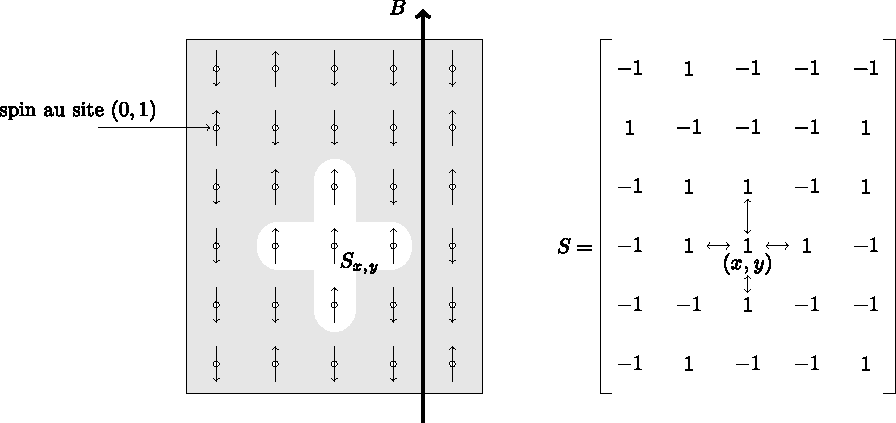
\includegraphics[width=0.85\linewidth]{TD3/schema_ising.pdf}
\caption{Représentation du modèle d'Ising sur un réseau carré fini, des interactions entre spins voisins et du champ magnétique externe. À droite, représentation numérique du modèle sous forme d'une matrice avec des valeurs $\pm 1$.}
\label{fig:schema_ising}
\end{figure}

L'idée est la même sur un réseau carré 3D ou sur un réseau hexagonal, mais l'indiçage des sites est différent et les propriétés physiques seront différentes. Stricto censu, la physique qui nous intéresse n'est présente que pour des systèmes infinis, mais si l'on veut simuler le système numériquement, il faut bien prendre un système fini (de taille aussi grande que possible). Aussi, pour diminuer les effets de bords, on prend des conditions périodiques aux limites.\\

Quel est l'état fondamental du modèle d'Ising ? Est-il dégénéré ? Quel lien peut-on faire avec la symétrie $\mathbb{Z}_2$ mentionnée auparavant ?\\

La physique de l'état fondamental n'est bien sûr pas celle de matériaux dans des conditions normales. Il faut prendre en compte la température $T$, qui va avoir tendance à désordonner notre système. À température finie et à champ $B$ nul, il va y avoir compétition entre l'énergie, qui cherche à être minimisée et donc à aligner les spins, et les fluctuations thermique (l'entropie) qui les désaligne, d'autant plus que la température est élevée. On alors tous les ingrédients pour observer une transition de phase.\\

La physique statistique nous enseigne que le système va explorer toutes les configurations $S\in\mathcal{C}$ possible, et la probabilité d'observer une configuration $S$ est donnée par la distribution de Boltzmann
\begin{equation}
P_{T,B}[S]=\tfrac{1}{Z({T,B})}\,\mathrm{e}^{-\beta \mathcal{H}_B[S]} \quad \text{où $Z$ est tel que} \quad \sum_{S\in\mathcal{C}}P_{T,B}[S] = 1
\end{equation}
avec $\beta=1/k_\mathrm{B}T$. On peut alors vouloir calculer, par exemple, la magnétisation moyenne du matériau (au sens probabiliste), qui est la valeur moyennée de $M[S]$ sur l’ensemble des configurations possibles :
\begin{equation}
\langle M\rangle_{T,B} = \sum_{S\in\mathcal{C}} M[S]\,P_{T,B}[S]
\end{equation}
Numériquement, on pourrait simplement parcourir toutes les configuations $S$ pour calculer $Z$ et cette valeur moyenne. Calculer le nombre de configurations pour un système de $10\times 10$. Est-ce faisable avant que la fin de vie du Soleil (compter $1\,\mathrm{ns}$ par évaluation de configuration) ?

\subsection{Algorithme de Metropolis pour échantilloner des configuration}

Pour résoudre le problème, il faut réaliser qu'il n'est pas nécessaire de parcourir toutes les configurations pour obtenir une valeur approchée de $\langle M\rangle$ ou d'autres observables. Il suffit la plupart du temps de considérer un sous-ensemble "typique" de notre ensemble canonique à $T,B$, dans le sens où les configurations hautement improbables ne contribuent pas à la moyenne.\\

Libérés de la contrainte de parcourir l’ensemble des configurations possibles, le plus simple est de parcourir aléatoirement l'espace des configurations : c'est l'esprit des méthodes de Monte-Carlo. Pour être efficace et considérer uniquement notre sous-ensemble "typique", on va parcourir l'espace des configurations tout en restant dans la "zone des configurations probables" : c'est l'esprit de l'\emph{échantillonage par chaînes de Markov}.\\

Le principe est simple : on part d'une configuration $S^{(0)}$ (peu importe laquelle), et on effectue une marche aléatoire pour obtenir une autre configuration $S^{(1)}$, puis $S^{(2)}$... de sorte qu'à chaque étape $k$, on augmente la probabilité $P_{T,B}[S^{(k)}]$ tout en autorisant de parfois aller explorer des configurations moins probables. L'objectif est que cette marche aléatoire produise au long terme un ensemble de configurations $\{ S^{(k)} \}_{k\leq K}$ ressemblant à l'ensemble complet :
\begin{equation}
\forall S\in\mathcal{C},\quad\lim_{K\to\infty} (\text{distrib. empirique de $S$ dans une chaine de longueur $K$}) = P[S] \label{eq:convergence-proba}
\end{equation}

Le lecteur intéressé par une idée moins vague et plus rigoureuse se reportera par exemple à l'article Wikipedia sur les \href{https://fr.wikipedia.org/wiki/M%C3%A9thode_de_Monte-Carlo_par_cha%C3%AEnes_de_Markov}{Méthode de Monte-Carlo par chaînes de Markov}.\\

Il n'est pas très difficile de montrer que l'algorithme suivant, l'\emph{algorithme de Metropolis}, produit bien une chaîne de Markov ayant cette propriété, et donc que les moyennes calculés convergent vers la moyenne d'ensemble canonique.\\

\begin{enumerate}
  \item \textbf{Proposition de transition}\\
  Ayant une configuration $S^{(k)}$, on propose une transition vers une autre configuration $S^\text{(prop)}$ choisie aléatoirement. Dans notre cas, le plus simple est de choisir un spin $i$ au hasard, selon une distribution uniforme, et d'inverser ce spin :
  \begin{equation*}
    S^\text{(prop)}_i = -S^{(k)}_i
  \end{equation*}
  Tous les autres sites resteront inchangés.\\

  \item \textbf{Calcul de la probabilité d’acceptation}\\
  Maintenant que l'on a proposé cette nouvelle configuration $S^\text{(prop)}$ (qui est similaire à un spin près), on accepte ou non cette proposition. Pour quantifier cela, on calcule la probabilité d’acceptation
  \begin{equation*}
    r = \min\left( 1, \frac{P_{T,B}[S^\text{(prop)}]}{P_{T,B}[S^{(k)}]} \right)
  \end{equation*}
  Dans le cas de l'ensemble canonique, elle est très simple car elle ne dépend que de la différence d'énergie interne :
  \begin{equation*}
    r = \min\left( 1, \mathrm{e}^{-\beta\,\Delta E} \right) \quad \text{avec} \quad \Delta E = \mathcal{H}_B[S^\text{(prop)}]-\mathcal{H}_B[S^{(k)}]
  \end{equation*}
  Si l’énergie interne baisse ($\Delta E < 0$), alors $r=1$ et on acceptera certainement cette proposition de transition. Sinon les fluctuations thermiques peuvent l'admettre avec une probabilité $r = \mathrm{e}^{-\beta\,\Delta E} < 1$.\\Étant donné $S^{(k)}$, représenté par l'objet \inline{S} de type \inline{Réseau}, et le site proposé \inline{Site i = S.site_aleatoire()}, écrire le bout de code (5 lignes !) calculant la probabilité d'acceptation.\\

  \item \textbf{Acceptation avec probabilité $r$}\\
  Enfin, la dernière étape concerne l'acceptation ou non de l’état proposé $S^\text{(prop)}$. Pour cela on tire aléatoirement un nombre $t$ dans une distribution uniforme sur $[0,1]$ et on le compare à la probabilité d'acceptation $r$ de l'état proposé que l’on vient de calculer :
  \begin{itemize}
    \item si $t<r$, alors l'état proposé $S^\text{(prop)}$ devient le nouvel état $S^{(k+1)}$ (dans notre cas, on inverse le spin $i$)
    \item sinon le nouvel état $S^{(k+1)}$ \emph{reste identique} à l'ancien état $S^{(k)}$ (ça ne veut pas dire qu'on ignore ce pas de l'algorithme, ça veut dire que $S^{(k)}$ comptera deux fois)
  \end{itemize}
  Il est facile de se convaincre que cette façon de faire revient à accepter la transition avec une probabilité $r$, et que prendre $r=\mathrm{e}^{-\beta\,\Delta E}$ au lieu de $r=\min(1,\dots)$ revient au même.\\

  \item \textbf{Calcul des observables}\\
  On ajoute cette nouvelle configuration $S^{(k+1)}$ dans nos moyennes empiriques, par exemple à l'aimantation. Bien sûr, on ne va pas stocker toutes les configurations explorées puis calculer les moyennes; on calcule les moyennes en vol ou on stocke les valeurs successives instantannées des observables.\\
\end{enumerate}

De façon figurée, on navigue aléatoirement dans le paysage formé par le hamiltonien, en cherchant à minimiser l'énergie (en "restant dans les vallées"), tout en autorisant l'exploration de zones de plus haute énergie, d'autant plus que la température est élevée. À température infinie ($\beta=0$), les transitions sont toujours acceptées et on voit bien que l'on tend vers un système totalement désordonné. À l'inverse, à faible température (haut $\beta$), il est rare que les transitions augmentant l'énergie soient acceptées car $\mathrm{e}^{-\beta\mathcal{H}}$ est très raide : on descend vers des configurations de basse énergie, proche d'un état fondamental.\\

Notez que l'algorithme de Metropolis n'est pas limité à l'échantillonage d'un ensemble canonique. C'est un algorithme très général qui permet d'échantilloner n'importe quelle distribution de probabilité, dans un espace quelconque. La généralité de cet algorithme a un prix : la vitesse de convergence vers la distribution cible (cf. eq. \ref{eq:convergence-proba}) est en général loin d'être optimale.

\subsection{Programmation}

On fixera l'échelle d'énergie et de température en fixant $J=k_\mathrm{B}=1$. Écrire une fonction
\begin{minted}[samepage]{c++}
bool ising_metropolis_step (Réseau& S, float beta, float B);
\end{minted}
effectuant un pas de l'algorithme de Metropolis. Si l'inversion de spin est acceptée, la fonction modifie \inline{S} et renvoie \inline{true}. Sinon, elle ne fait rien et renvoie \inline{false}. Encore une fois, la description de l'algorithme peut être intimidante, mais cette fonction tient en moins de 20 lignes de code. Est-ce nécessaire de passer \inline{S} par référence ?\\

Pour tirer un nombre aléatoire entre 0 et 1, on pourra déclarer un générateur et une distribution uniforme ainsi :
\begin{minted}[samepage]{c++}
#include <random>
std::mt19937 rng;
std::uniform_real_distribution<float> distrib_u01 (0,1);
\end{minted}
et obtenir une valeur ainsi : \inline{float t = distrib_u01(rng);}\\

\begin{correction}
\begin{minted}[samepage]{c++}
bool ising_metropolis_step (Réseau& S, float beta, float B) {
  // choix d'un site aléatoire
  Site i = S.site_aleatoire();

  // calcul du champ local
  int8_t b = 0;
  for (Site j : S.voisins(i))
    b += S[j];

  // différence d'énergie locale sous inversion du spin
  float dE = 2 * S[i] * (B + b);

  // inversion du spin avec probabilité d'acceptation
  float r_flip = exp( -beta * dE );
  if (distrib_u01(rng) < r_flip) {
    S[i] = -S[i];
    return true; // spin inversé (transition acceptée)
  }
  else
    return false;
}
\end{minted}

\end{correction}

Il ne reste plus qu'à écrire la boucle principale du programme. Initialisez une configuration où chaque site est de valeur aléatoire $\pm 1$. Ensuite, écrivez une boucle (infinie pour le moment) où vous effectuez un pas de l'algorithme de Metropolis. Pour l'instant, on ne calcule aucune observable. Contentez-vous d'afficher la configuration instantannée (disons tous les $10^6$ pas pour ne pas ralentir trop le programme). On commencera avec $B=0$ et en se plaçant quelque part autour de la température critique, qui vaut
\begin{equation}
\beta_\text{c}^\square = \frac{\ln(1+\sqrt{2})}{2}
\end{equation}
pour un réseau carré en deux dimensions (résultat analytique difficile à obtenir, Lars Onsager en 1944). Pour un réseau hexagonal ou triangulaire, la température critique (qui est un résltat analytique relativement simple à calculer par dualité\footnote{Il s'agit d'un argument magnifique de dualité entre le réseau triangulaire et hexagonal. On pourra par exemple consulter \url{http://chimera.roma1.infn.it/ENZO/FC/ESTRATTI/DUALITY/mussardo_duality.pdf}, partie 4.3. Le résultat pour le réseau hexagonal est en dernière page, où $L=J$. On a bien
\begin{equation}
\sinh(2\,J\,\beta_\text{c})=\sqrt{3} \quad \xLeftrightarrow[J=1]{} \quad \beta_\text{c} = \frac{\ln(2+\sqrt{3})}{2}
\end{equation}
}) est donnée respectivement par
\begin{equation}
\beta_\text{c}^\triangle = \frac{\ln(3)}{4} \quad\text{et}\quad \beta_\text{c}^{\hexago} = \frac{\ln(2+\sqrt{3})}{2}
\end{equation}

Une taille raisonnable de système est $200 \times 100$. Pour ceux affichant le système dans le terminal, n'hésitez pas à dézoomer fortement ou réduire la taille de la police de caractères pour voir le système dans son entièreté. Pour ceux ayant mis en place l'affichage graphique, un système de $300 \times 300$ est envisageable. Enfin, pour garantir une bonne performance malgré les couches d'abstraction, on compilera avec les option \inline{-Ofast -flto} (à la fois à la compilation et à l'édition de liens).\\

\begin{correction}
Voilà un exemple du programme principal. La fonction \inline{ising_metropolis_step} est déclarée directement dans le \filename{main.cpp}, mais il est préférable d'avoir une paire de fichiers \filename{ising.h}/\filename{ising.cpp} séparée. On a implémenté à la fois l'affichage dans la console et avec la SFML dans une fenêtre.
\begin{minted}[fontsize=\footnotesize]{c++}
#include "reseau_carre.h"
#include <random>
#include <iostream>
#include <SFML/Graphics.hpp>

std::mt19937 rng (42);
std::uniform_real_distribution<float> distrib_u01 (0,1);

bool ising_metropolis_step (Réseau& S, float beta, float B) {
  ...
}

int main () {

  // on demande la valeur de la température et du champ à l'utilisateur
  float T_sur_Tc;
  std::cout << "T/Tc ?" << std::endl;
  std::cin >> T_sur_Tc;
  float beta = log(1+sqrt(2))/2 / T_sur_Tc;
  std::cout << "B ?" << std::endl;
  float B;
  std::cin >> B;

  Réseau S (200, 100);

  // initialisation du système : valeurs aléatoires
  for (int x = 0; x < S.nx; x++) {
    for (int y = 0; y < S.ny; y++) {
      Site i = S.site_xy(x,y);
      S[i] = 2 * (rng()%2) - 1;
    }
  }

  sf::RenderWindow window (sf::VideoMode(2*S.nx,2*S.ny), "Ising");

  while (true) {

    // 10^6 pas de l'algorithme de Metropolis pour le modèle d'Ising
    for (int n = 0; n < 1000000; n++) {
      ising_metropolis_step(S, beta, B);
    }
    
    // Affichage dans la console
    S.affiche_console();

    // Affichage graphique
    window.clear(sf::Color::White);
    S.affiche_SFML(window, 0, 0);
    window.display();

  }

  return 0;
}
\end{minted}
\end{correction}

Pour savoir si votre code fonctionne, vous devriez observer un système totalement désordonné (comme de la neige sur les télévisions analogiques) pour $T \gg T_\text{c}$, et une formations de gros domaines évoluant peu (voire d'un système uniforme) pour $T \ll T_\text{c}$ (cf. fig. \ref{fig:configs_ising}). Qu'observez-vous à $T \simeq T_\text{c}$, et comment décririez-vous la structure spatiale ? À quel point le système est-t-il sensible au champ $B$ appliqué, en fonction de $T/T_\text{c}$ ?\\

Notons enfin que, en observant l'évolution de notre système au cours de la simulation, on a l'impression d'observer la dynamique temporelle (au sens des équations du mouvement). Certains comportements, comme le déplacement des frontières de domaines magnétiques, sont en effet réalistes. Ce n'est pas surprenant car les transitions proposées dans notre algorithme sont \emph{locales}, comme les équations du mouvement. Mais ne vous y méprenez pas : ce n'est pas parce que c'est réaliste que la dynamique est correctement simulée\footnote{Ce n'est en effet pas le cas, et certains aspects ne sont pas reproduits, comme la notion de \emph{ralentissement critique} lorsque l'on approche de la transition de phase.}. Il ne faut pas perdre de vue que notre algorithme n'est rien d'autre qu'un générateur aléatoire de configurations ! \emph{Seules les moyennes calculées à partir de cette suite de configuration sont garanties d'avoir un sens.}

\begin{figure}[H]
\centering

\includegraphics[width=0.48\linewidth]{TD3/T_sur_Tc_1.3.png}
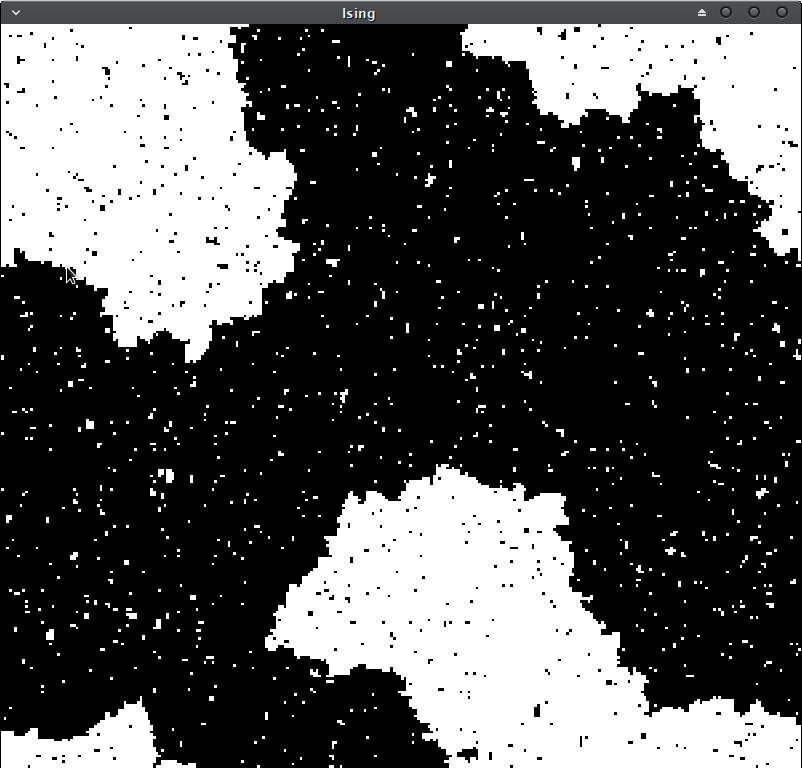
\includegraphics[width=0.48\linewidth]{TD3/T_sur_Tc_0.8.png}
\caption{Configurations typiques du modèle d'Ising pour $T = 1.3\, T_\text{c}$ (droite) et pour $T = 0.8\, T_\text{c}$ (gauche, après un temps fini de simulation). $B=0$ dans les deux cas.}
\label{fig:configs_ising}
\end{figure}

\begin{correction}
À $T \simeq T_\text{c}$, les bords de domaine ont l'air très "déchiquetés" et ne sont pas nets. Le système a en fait un aspect fractal : on a des domaines de toutes tailles, des plus petits aux plus gros et s'interpénétrant. On verra dans la suite qu'on a en effet une invariance d'échelle au point critique.\\

On remarque que le système fluctue beaucoup. De plus, il devient très sensible au champ magnétique : à $T = 0.98 \, T_\text{c}$, il suffit de $B=\pm 0.001$ pour forcer le système à s'aligner sur le champ. Au contraire, plus on s'éloigne de $T_\text{c}$, moins le champ influence le système.\\

Voilà deux configurations typiques aux point critique pour un réseau carré à gauche et hexagonal à droite :
\begin{center}
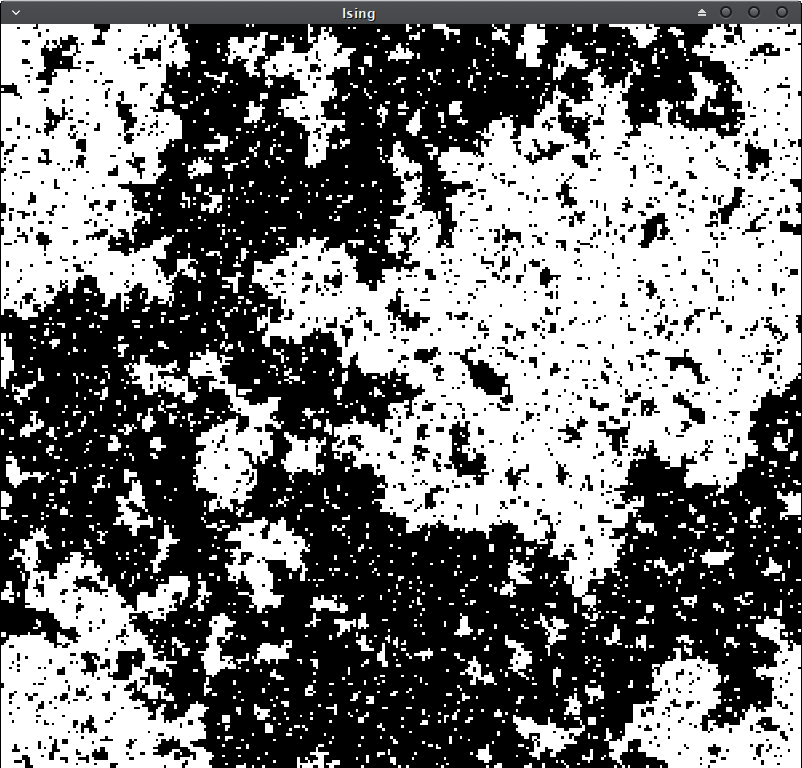
\includegraphics[height=0.46\linewidth]{TD3/T_sur_Tc_1.0.png}
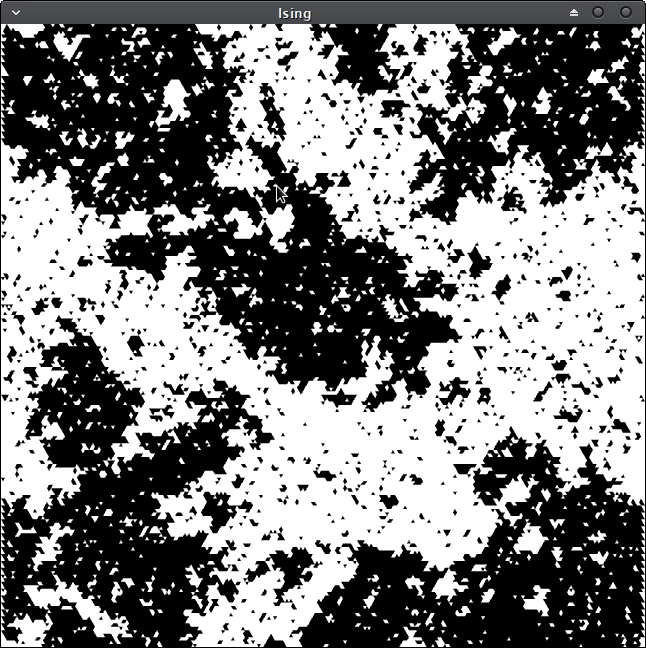
\includegraphics[height=0.46\linewidth]{TD3/T_sur_Tc_1.0_hexa.png}
\end{center}
On ne remarque pas de différences structurelles entre réseaux carrés, triangulaires ou haxagonaux, et c'est bien normal : proche du point critique, les détails microscopiques du système ne comptent plus, et les comportements relatifs au point critique sont identiques. Seule $T_\text{c}$ change. On dit que ces systèmes appartiennent à la même \emph{classe d'universalité}.
\end{correction}

\subsection{Calcul de quelques observables}

On va maintenant calculer quelques observables en fonction de $T$ et $B$. En réalité, comme le changement est faible de $S^{(k)}$ à $S^{(k+1)}$, il n'est pas nécessaire de re-calculer les observables (ce qui est lourd) à chaque pas : on se contentera de le faire tous les $10^4$ pas pour ne pas ralentir trop le programme\footnote{Une alternative serait de mettre à jour les observables d'intérêt à chaque pas de façon plus intelligente : lorsqu'un spin est inversé, il n'y a pas besoin de re-parcourir tout le réseau pour calculer l'énergie ou la magnétisation, il suffit d'appliquer la différence d'énergie $\Delta E$ et la différence de magnétisation $\Delta  M=\pm 2$. Mais ce n'est en réalité pas nécessaire. En effet, les configurations successives sont (malheureusement) fortement corrélées dans notre cas, et toutes les prendre en compte n'apporterait aucune précision statistique supplémentaire.}.\\

Écrire une fonction prenant un \inline{const Réseau& S} et $B$, et renvoyant un tuple contenant l'énergie instantannée et la magnétisation instantannée. On renvoiera des quantités intensives $M/N\in[-1,1]$ et $E/N$ en divisant la magnétisation et l'énergie totale par le nombre de sites.

\begin{correction}
\begin{minted}[samepage,fontsize=\footnotesize]{c++}
std::tuple<float,float> ising_magnétisation_énergie (const Réseau& S, float B) {
  int M = 0;
  float E = 0;

  for (int x = 0; x < S.nx; x++) {
    for (int y = 0; y < S.ny; y++) {
      Site i = S.site_xy(x,y);

      // magnétisation
      M += S[i];

      // énergie
      for (Site j : S.voisins(i)) 
        E -= S[i] * S[j] / 2.f;
      E -= S[i] * B;

    }
  }

  int ntot = S.nx * S.ny;
  return { M /(float) ntot, E / ntot };
}
\end{minted}
\end{correction}

Enfin, écrivez les valeurs instantannées des observables ainsi que le nombre de pas effectués dans un fichier texte pour pouvoir ensuite afficher les courbes dans un outil externe. Vous pouvez vous inspirer du code suivant :

\begin{minted}[samepage,fontsize=\footnotesize]{c++}
std::ofstream fichier_r ("ising_magnétisation_énergie.txt");

while (steps < 1000000000) {

  if (steps%10000 == 0) {
    auto [m, e] = ising_magnétisation_énergie(S, B);
    fichier << steps << " " << m << " " << e << std::endl;
  }

  ising_metropolis_step(S, beta, B);
  steps++;

  ...
}
\end{minted}

N'hésitez pas à effectuer jusqu'à $10^8$ ou $10^9$ pas de l'algorithme pour un système de $200 \times 100$. Enregistrez quelques réalisations (au moins 2 ou 3) pour un même $(T,B)$ de votre choix, et affichez les courbes avec un outil externe de votre choix. Le code Python suivant permet d'ouvrir quelques fichiers \filename{ising\_magnétisation\_énergie.$N$.txt} et d'afficher les courbes de façon superposée :
\begin{minted}[samepage,fontsize=\footnotesize]{python}
import numpy as np
import matplotlib.pyplot as plt
fig, (ax1,ax2) = plt.subplots(2,1, figsize=(8,8), sharex=True)
for i in range(nombre_de_fichiers):
    data = np.loadtxt(f"ising_magnétisation_énergie.{i}.txt")
    steps = data[:,0]
    magnet = data[:,1]
    énergie = data[:,2]
    ax1.plot(steps, magnet, alpha=0.7)
    ax2.plot(steps, énergie, alpha=0.7)
ax1.set_ylim(-1,1)
ax1.set_ylabel("Magnétisation")
ax2.set_ylabel("Énergie interne")
ax2.set_xlabel("Nombre de pas de l'algorithme")
\end{minted}

À partir de combien de pas de l'algorithme considérez-vous que les configurations deviennent "typiques" ? Selon vous, est-ce que cela dépend de la taille de système choisie ? Pourquoi ? Que faut-t-il faire, avec d'une telle suite de valeurs instantannées $O^{(k)}$, pour calculer nos valeurs moyennes $\langle O \rangle_{T,B}$ ?

\begin{correction}
La figure suivante montre quelques réalisations à $T=T_\text{c}$ et $B=0$ pour un système de taille $200 \times 100$. On remarque que le taux d'acceptation et l'énergie convergent vers leurs valeurs asymptotiques en quelques $10^7$ pas, c'est-à-dire en quelques centaines de pas par site. Ce comportement est relativement indépendant de $T$ et $B$. Par contre, la magnétisation, qui est le paramètre d'ordre de notre système, ne semble ici pas se stabiliser avant $\sim 10^8$ pas, et on observe d'ailleurs deux asymptotes\footnote{Ceux familiers avec la physique des transitions de phases devraient s'en étonner : il ne devrait pas y avoir de forte magnétisation spontannée à $T=T_\text{c}$, mais seulement en dessous. Il s'agit en fait d'un effet de taille finie, qui a tendance à déplacer la température critique effective (ici vers $1.02 \sim 1.05 \,T_\text{c}$) et à rendre la transition de phase floue, d'autant plus que le système simulé est petit. L'effet se réduit en augmentant la taille du système.}. Cette lenteur de convergence se trouve exacerbée pour $T \leq T_\text{c}$ en général, à cause de la brisure d'ergodicité (le paysage énergétique voit apparaître des vallées très séparées, et l'algorithme a du mal à explorer toutes les configurations possibles en un temps fini). Bien sûr, plus le système est grand et plus la convergence sera lente car l'espace des configurations grossit exponentiellement.\\

On remarque aussi et surtout que les configurations successives sont fortement corrélées, ce qui est décevant pour un générateur aléatoire de configurations ! Il va donc falloir faire tourner l'algorithme longtemps, et surtout effectuer de nombreuses réalisations avec des conditions initiales différentes pour espérer faire justice à l'ensemble des configurations possible.\\
\begin{center}
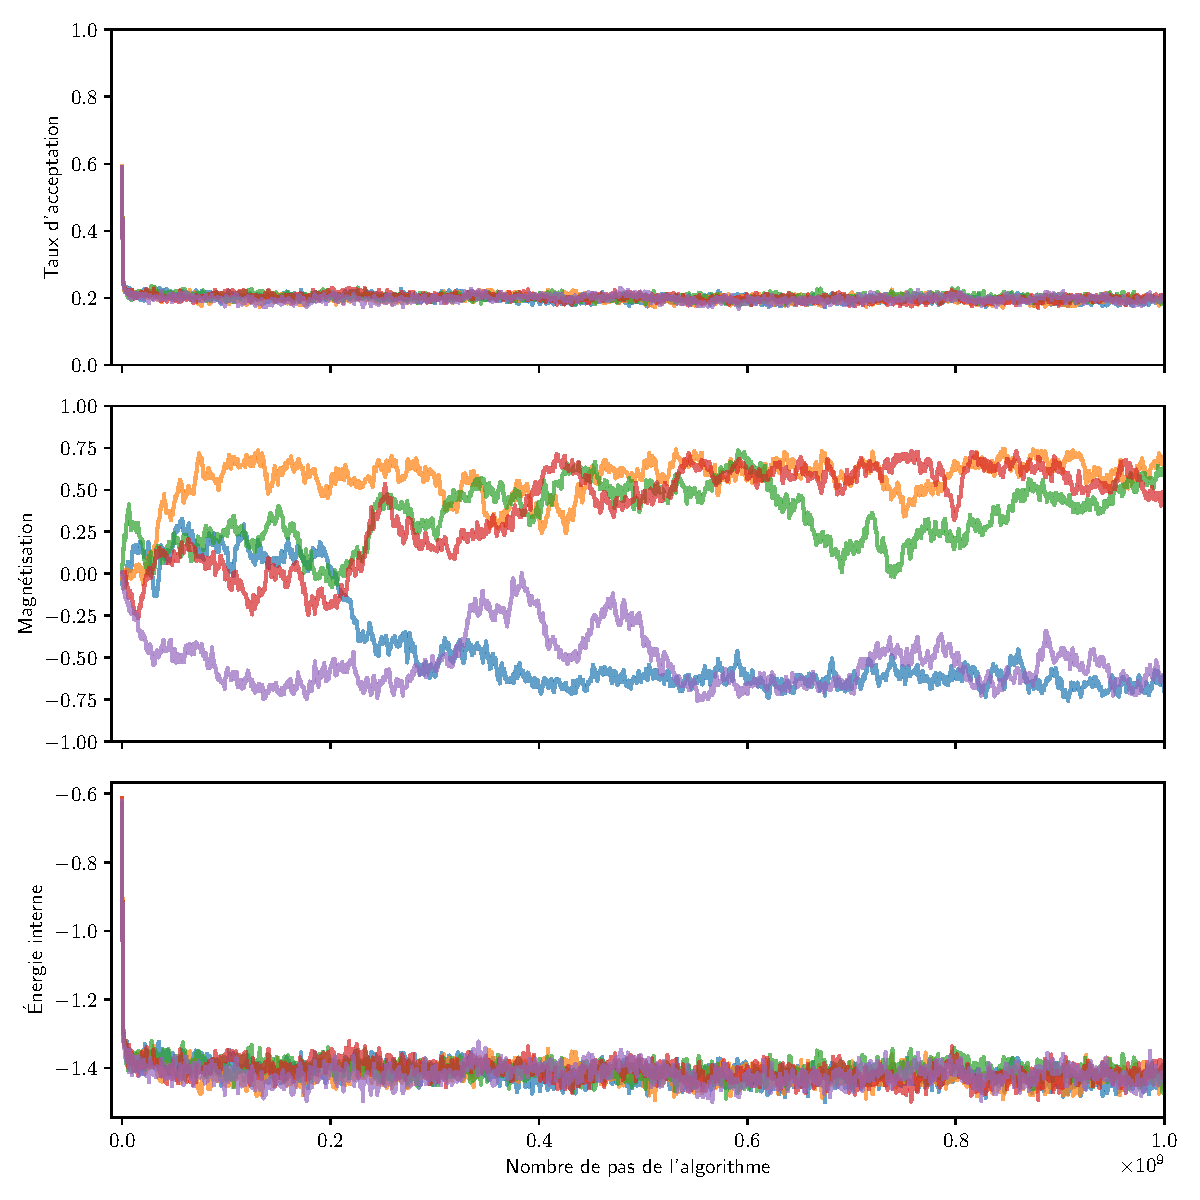
\includegraphics[width=1\linewidth]{TD3/ising_stats_courbes_T1_B0_nx200_ny100.pdf}
\end{center}
Enfin, pour calculer notre moyenne $\langle O \rangle_{T,B}$, on va éliminer (dans notre cas) les premiers $\sim 10^8$ pas :
\begin{equation*}
\langle O \rangle_{T,B}^\text{réalisation} = \frac{1}{N-10^8} \sum_{k=10^8}^{N} O^{(k)}
\end{equation*}
Il semble qu'on ne puisse même pas calculer la vraie moyenne d'ensemble $\langle O \rangle_{T,B}$ à partir d'une seule réalisations, et c'est en fait une chose heureuse. En effet, comme on va le voir par la suite, la moyenne d'ensemble de la magnétisation est toujours nulle par symétrie $\mathbb{Z}_2$, et ça nous arrange bien qu'une réalisation n'explore qu'une seule magnétisation (positive ou négative) dans le temps fini de la simulation. Mais c'est un point délicat dans lequel nous n'allons pas nous engouffrer...
\end{correction}


\subsection{Étude de la transition de phase}

On peut maintenant étudier la transition de phase. Nous allons d'abord fixer $B=0$ et observer la magnétisation en fonction de la température $T$ autour de la température critique, par exemple $T=\{0.95,0.975,1,1.025,1.05,1.1\}\,T_\text{c}$. Pour cela, nous allons faire tourner le programme plusieurs fois, avec une valeur de $T$ différente à chaque réalisation, et enregistrer un fichier pour chaque réalisation. Pour automatiser la chose, on pourra utiliser un programme de la forme :
\begin{minted}[fontsize=\footnotesize]{c++}
int main () {

  for (int i_T = 0; i_T < 6; i_T++) {

    float T_sur_Tc = 0.95 + 0.025 * i_T;
    float beta = log(1+sqrt(2))/2 / T_sur_Tc;
    float B = 0;

    std::cout << "---------" << std::endl;
    std::cout << "T = " << T_sur_Tc << ", B = " << B << std::endl;

    std::string nom_fichier = std::string("scan_T/ising_magnétisation_énergie.") + std::to_string(k) + ".txt";
    std::ofstream fichier_r (nom_fichier.c_str());

    Réseau S (..., ...);

    ...

  }
\end{minted}
qui créera une suite de fichiers dans le dossier \filename{scan\_T} que l'on aura créé au préalable. Dans votre programme d'analyse de données, calculez les moyennes, ainsi que les écarts-type (c'est-à-dire les fluctuations), pour chaque réalisation. Affichez un graphe de la magnétisation en fonction de la température, en représentant les fluctuations par des barres d'erreur. Affichez aussi un graphe des fluctuations d'énergie et de magnétisation en fonction de $T/T_\text{c}$.\\

Commentez la courbe $M(T)$. Comparez éventuellement avec vos voisins. En quoi peut-on dire qu'il y a magnétisation spontannée pour $T < T_\text{c}$ ? Est-ce le cas pour toutes les réalisations ? Qualifiez ce que l'on voit en terme d'ordre et de désordre, et de compétition entre alignement des spins et entropie. Que se passe-t-il pour les fluctuations d'énergie et de magnétisation proche du point critique, et pourquoi ? Effectuez l'analogie avec le phénomène d'opalescence critique. Quel observable pourrions-nous utiliser pour quantifier l'ordre global du système ?\\

\begin{correction}
Le code Python suivant
\begin{minted}[fontsize=\footnotesize]{python}
import numpy as np
import matplotlib.pyplot as plt

T = []
M = []
varM = []
E = []
varE = []

for k in range(50):
    data = np.loadtxt(f"scan_T_big/ising_magnétisation_énergie.{k}.txt")
    steps = data[:,0]

    # on jette les premiers 10^9 pas :
    N0 = np.searchsorted(steps, 1e9)
    steps = data[N0:,0]
    magnet = data[N0:,1]
    énergie = data[N0:,2]

    T += [ 1.2 - 0.4*k/50. ]
    # calcul des moyennes :
    M += [ np.mean(magnet) ]
    varM += [ np.std(magnet) ]
    E += [ np.mean(énergie) ]
    varE += [ np.std(énergie) ]

fig, ((ax11, ax21), (ax12, ax22)) = plt.subplots(2,2, height_ratios=[2,1], figsize=(10,6.5), sharex=True)

ax11.scatter(T, E, marker='o', color='crimson')
ax11.set_ylabel(r"Énergie $\langle E \rangle$ par site")
ax12.scatter(T, varE, marker='o', color='crimson')
ax12.set_ylabel(r"Fluctus. $\langle E^2 \rangle - \langle E \rangle^2$ par site")
ax12.set_ylim(0,None)

ax21.errorbar(T, M, yerr=varM, linestyle='', marker='o', color='blue')
ax21.axhline(y=0, color='black')
ax21.set_ylim(-1,1)
ax21.set_ylabel(r"Magnétisation $\langle M \rangle$ par site")
ax22.scatter(T, varM, marker='o',  color='blue')
ax22.set_ylim(0,None)
ax22.set_ylabel(r"Fluctus. $\langle M^2 \rangle - \langle M \rangle^2$ par site")

ax12.set_xlabel(r"$T/T_\mathrm{c}$")
ax22.set_xlabel(r"$T/T_\mathrm{c}$")

plt.tight_layout()
fig.subplots_adjust(hspace=0.03)
\end{minted}
qui est pour un scan de 50 points de température, permet de produire la figure suivante (réseau carré de $250 \times 250$, $5\cdot 10^9$ pas de simulation) :
\begin{center}
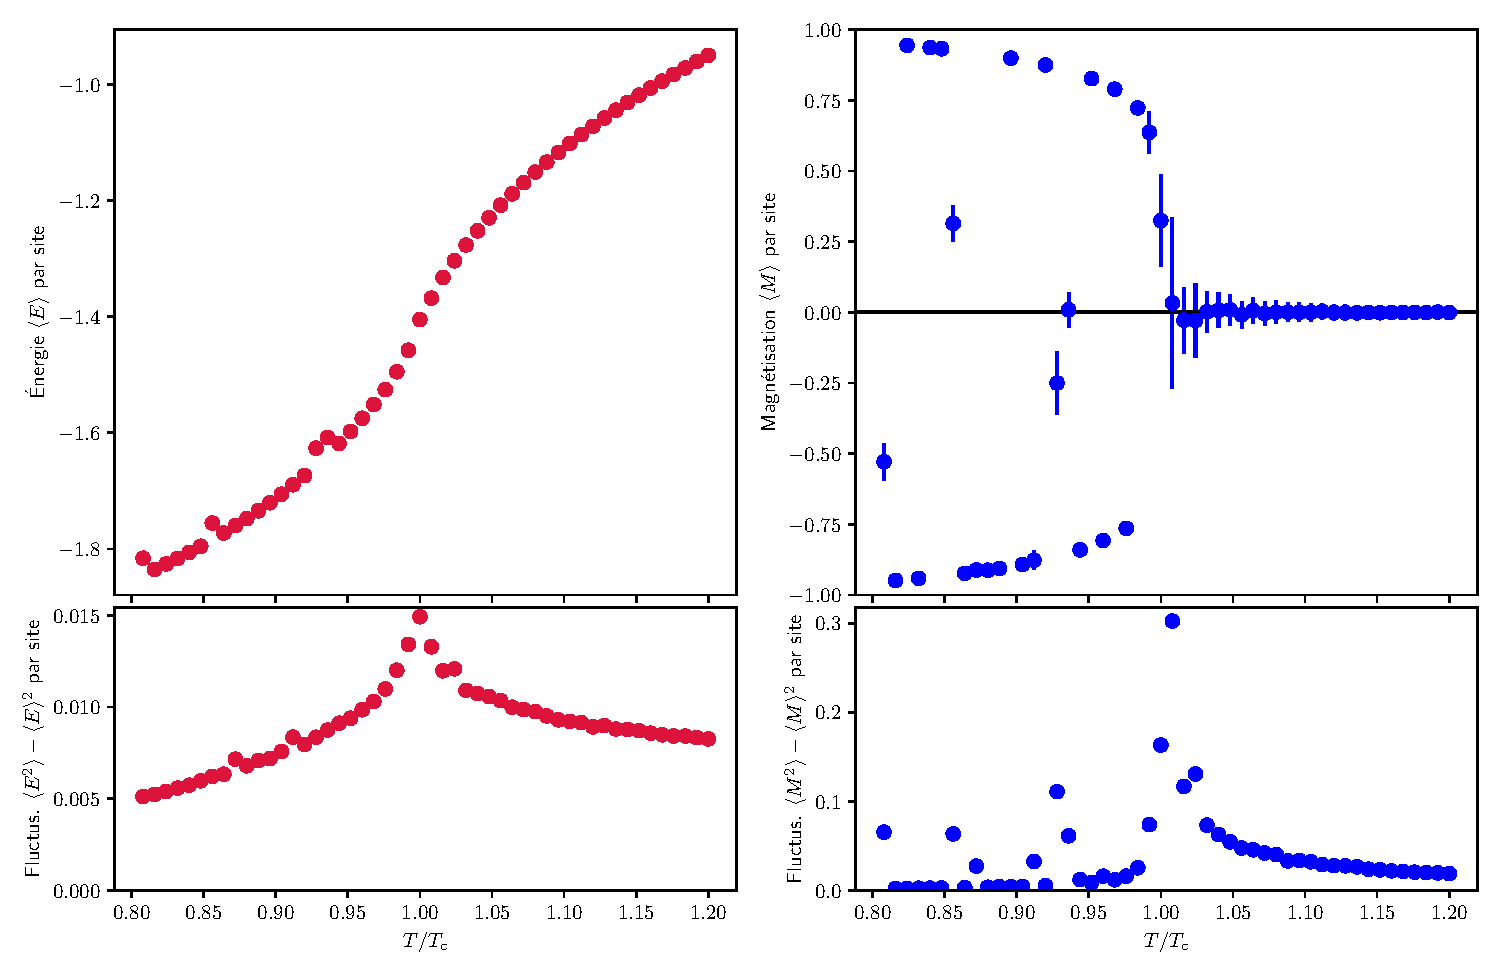
\includegraphics[width=1\linewidth]{TD3/ising_stats_scanT_250x250_5e9steps_pasdécoupé.pdf}
\end{center}

Commençons par le plus simple. L'énergie interne diminue avec la température, ce qui n'est pas surprenant : plus la température est faible, moins les fluctuations agissent et plus le système peut s'approcher de l'état fondamental, qui a une énergie de $-2$ par site pour un réseau carré.\\

\begin{enumerate}
\item Pour $T > T_\text{c}$, on observe une magnétisation nulle : même si les spins cherchent à s'aligner de voisins en voisins, les fortes fluctuations thermiques font qu'ils y a de nombreuses zones du système de magnétisation aléatoire, donnant une moyenne nulle à la magnétisation globale. Dans la compétition énergie/entropie, c'est l'entropie qui domine.

\item En s'approchant de la température critique, les fluctuations thermiques diminuent et on observe des domaines magnétiques de plus en plus gros, qui se compensent de moins en moins : les fluctuations de la magnétisation globale deviennent de plus en plus importantes. À la température critique, les spins commencent à s'aligner à l'échelle du système entier, et une magnétisation globale apparaît vite à mesure que l'on diminue la température.

\item Pour $T < T_\text{c}$, le système s'aligne entièrement et spontanément : il y a \emph{brisure spontannée de la symétrie} $S \to -S$, et on observe une magnétisation globale non nulle à temps fini. Elle est parfois positive, parfois négative, d'où la présence des deux branches sur la courbe $M(T)$. Dans la compétition énergie/entropie, c'est l'énergie qui domine.
\end{enumerate}

Il s'agit d'une transition de phase, qui est d'autant plus nette que le système simulé est grand, et $\langle M \rangle$, ou plutôt $\langle |M| \rangle$, décrit à quel point le système s'ordonne dans son ensemble (on parle de \emph{paramètre d'ordre}, et d'ordre à longue portée lorsque $\langle |M| \rangle > 0$).\\

Dans nos simulations, on remarque aussi que le système n'arrive pas à complètement se magnétiser pour $T < T_\text{c}$, surtout à basses température. La raison est simple : en un temps fini, les domaines magnétiques qui se forment depuis la configuration aléatoire initiale n'ont pas le temps de se battre pour savoir qui gagne, d'autant plus que les faibles fluctuations thermiques ralentissent la dynamique du système et que le système est grand. Il faut alors moyenner plus longtemps et/ou effectuer plus de réalisations. Voici une courbe de $\langle |M| \rangle$ avec plus de réalisations :\\
\begin{center}
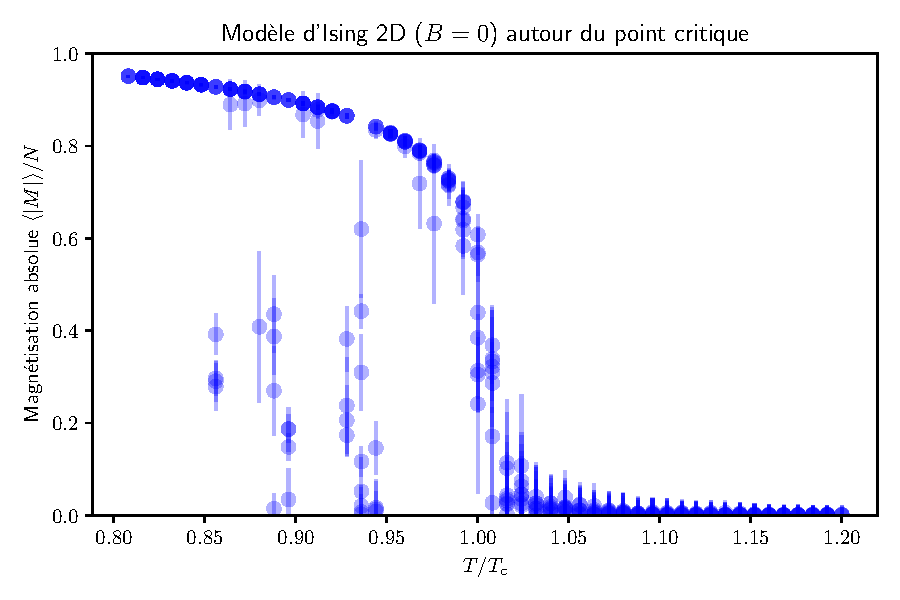
\includegraphics[width=0.75\linewidth]{TD3/ising_stats_scanT_250x250_5e9steps_2runs.magnetisation.pdf}
\end{center}

Quand aux fluctuations de magnétisation, elles sont maximales au point critique, ce qui est facile à comprendre : le système est sur le point de se magnétiser spontanément, mais dans la compétition énergie/entropie personne n'arrive à gagner. La moindre fluctuation change fortement la magnétisation à l'échelle du système entier. On remarque que le maximum de fluctuations d'énergie se trouve légèrement en dessous de la température critique, ce qui est attendu pour un système de taille fini.
\end{correction}

Si il vous reste du temps, il est instructif de se placer juste en dessous de la température critique et de faire tourner le programme (très) longtemps, puis d'afficher un histogramme des valeurs instantannées de la magnétisation. Quelle forme a-t-il ? En quoi est-ce une bien meilleure idée de regarder l'histogramme plutôt que la valeur moyenne $\langle M \rangle$ pour trouver la valeur exacte de la température critique (pensez à la symétrie d'inversion $S \to -S$ et à la conséquence immédiate que ça doit avoir sur la valeur de $\langle M \rangle$) ?

\begin{correction}
Sont tracées ici les histogrammes de magnétisation après accumulation sur plus de $10^9$ pas, et pour des températures très proches du point critique (la température diminue de gauche à droite) :
\begin{center}
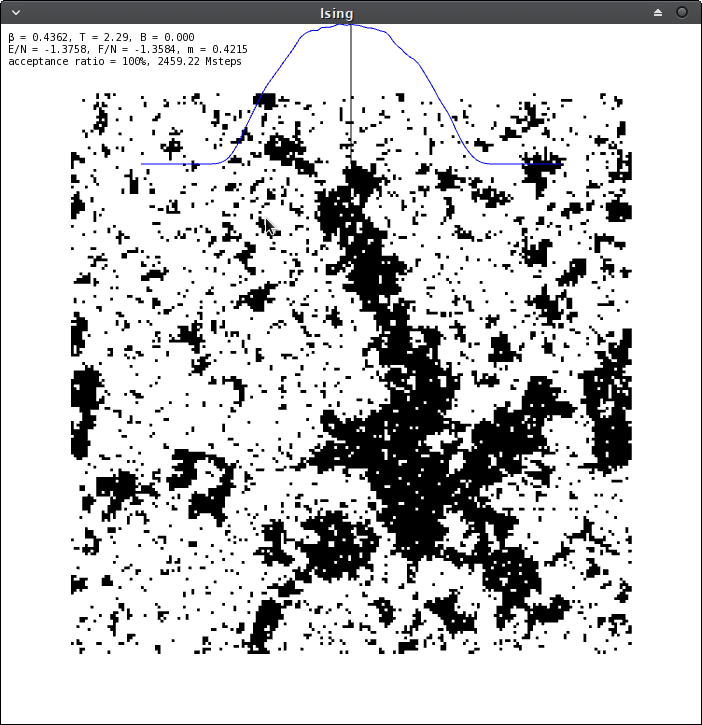
\includegraphics[width=0.32\linewidth]{TD3/histo_mag_2.png}
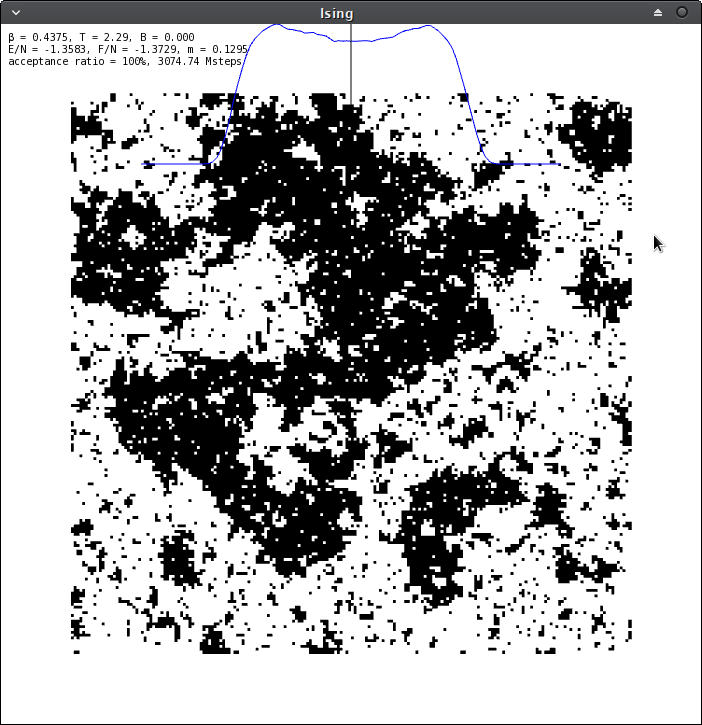
\includegraphics[width=0.32\linewidth]{TD3/histo_mag_3.png}
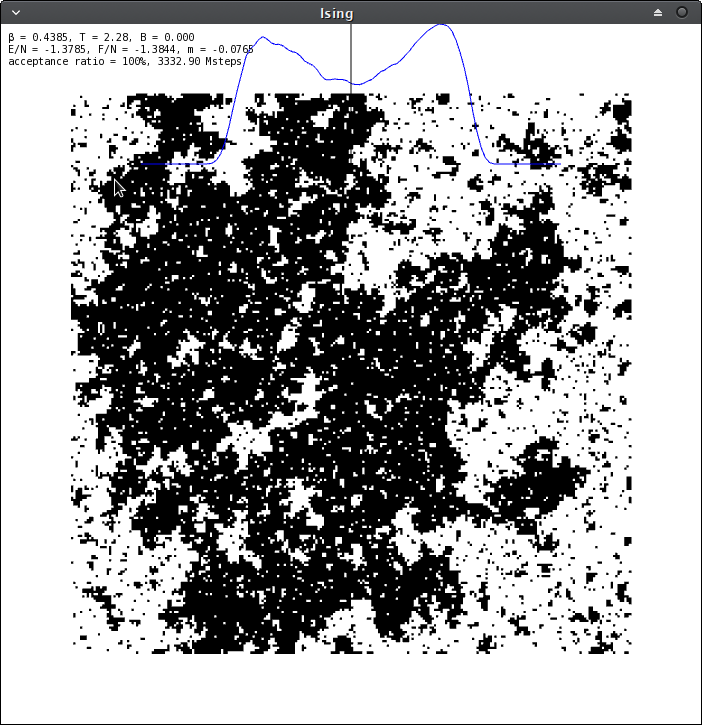
\includegraphics[width=0.32\linewidth]{TD3/histo_mag_4.png}
\end{center}
Dans les trois cas, on obtiendrait une magnétisation moyenne nulle ou presque car l'histogramme est symétrique autour de $M=0$ (ce qui n'est pas surprenant à cause de la symétrique d'inversion $S \to -S$) : on ne verrait pas clairement l'établissement spontannée d'une magnétisation alors qu'elle a lieu, et il est difficile d'établir la position exacte du point critique en regardant $\langle |M| \rangle$. On voit bien mieux ce qu'il se passe sur les histogrammes : pour $T < T_\text{c}$, la distribution s'élargit et devient bimodale, signe que le système se magnétise spontannément. Exactement à $T_\text{c}$, l'histogramme est plat autour de $M=0$ (c'est une autre façon de comprendre le fait que les fluctuations de magnétisation sont fortes).\\

Lorsque la température devient suffisemment faible, le système passe rarement ou presque jamais d'une magnétisation à l'autre le temps de la simulation car la barrière de potentiel est trop haute, et n'en choisit qu'une seule. C'est la \emph{brisure d'ergodicité} (le système n'explore plus tout l'espace des configurations en un temps fini).
\end{correction}

\subsection{[Bonus] Champ magnétique et hystérésis}

Tracez des courbes d'aimantation en fonction du champ magnétique $B$, pour trois températures : un peu en dessous de la température critique ($0.8\,T_\text{c}$ par exemple), au point critique, et au dessus de la température critique ($1.2\,T_\text{c}$ par exemple). Cette fois, il n'est pas utilise de faire tourner la simulation longtemps ($10^7$ pas par point suffisent). Pour étudier l'effet de mémoire du système\footnote{Sans perdre de vue qu'une simulation par échantillonage Monte-Carlo n'est pas forcément un outil adapté ni pertienent pour l'étude temporelle du système. Les effets de mémoire observés ici peuvent être considérés comme un artefact du fait qu'on utilise une proposition de transition locale, et doivent être considérés comme qualitatifs uniquement.}, au lieu de ré-initialiser la simulation à chaque $B$, on va simplement garder la configuration précédente et changer $B$ en vol. Faites une courbe pour $B$ montant de $-0.2$ à $+0.2$, puis pour $B$ descendant de $+0.2$ à $-0.2$. Commentez.

\begin{correction}
Voilà le résulat, obtenu avec un réseau carré de $200 \times 200$ (le résultat devrait être similaire quelque soit le réseau) :
\begin{center}
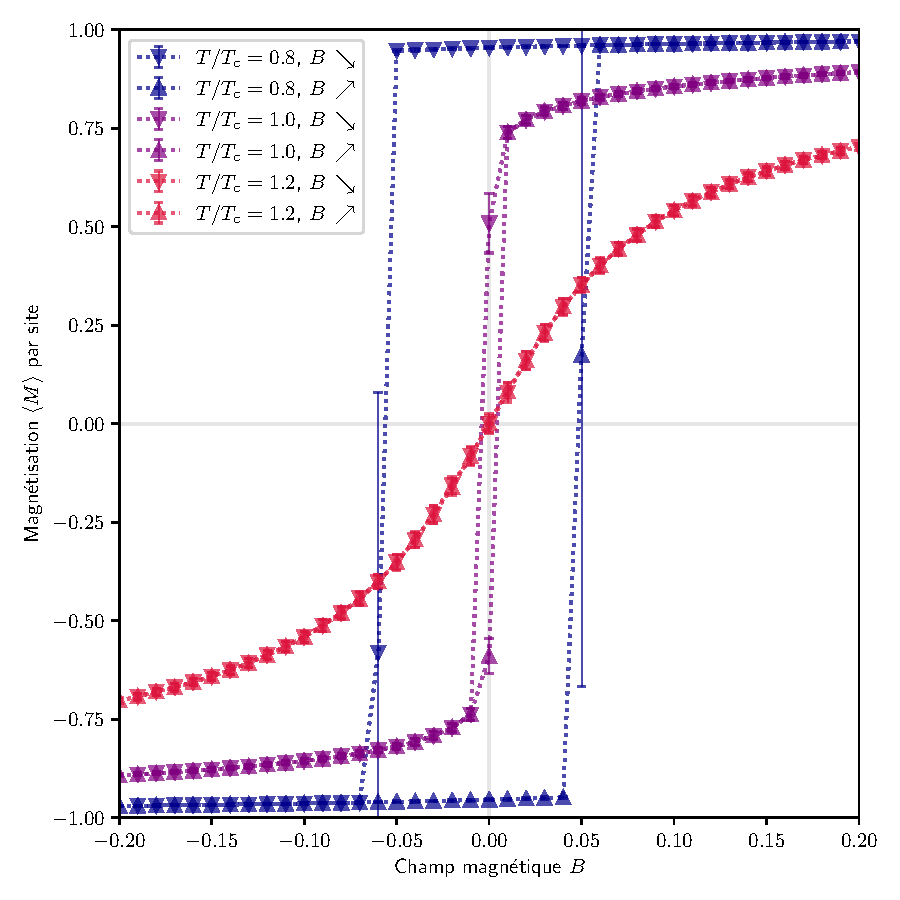
\includegraphics[width=0.75\linewidth]{TD3/ising_stats_scanB_updown_200x200_3T.pdf}
\end{center}
Les barres d'erreurs représentent ici la variance de la série de magnétisation de chaque incrément de $B$ ($10^8$ pas par incrément). Le code Python est disponible dans \filename{TD3/ising\_stats\_scanB.ipynb}.
\begin{enumerate}
\item Pour $T>T_\text{c}$, on observe une courbe lisse (en forme de "fonction d'activation") et indépendante du sens de variation de $B$. Il n'y a ici pas de magnétisation spontannée, il s'agit seulement de la polarisation des spins (certes aidée par les interactions) dans le champ magnétique, avec saturation à fort champ.
\item Pour $T=T_\text{c}$, on observe encore une courbe (presque) lisse, mais beaucoup plus raide autour de $B$. C'est parce que le système est beaucoup plus polarisable au point critique car le système est au bord de la magnétisation spontannée. Théoriquement, la pente est même infinie et la susceptibilité magnétique $\chi_\text{m}=\partial M \ \partial B$ est infinie à $T=T_\text{c}$, $B=0$. Le petit hysteresis observable provient du fait que, pour un système de taille finie, la température critique théorique est en fait un tout petit peu en dessous de la température critique réelle. Notre mesure est d'ailleurs d'un autre moyen pour trouver la position précise du point critique.
\item Pour $T<T_\text{c}$, il y a magnétisation spontannée, et il faut appliquer un champ fini (ici $B_\text{c}(T) \approx \pm 0.05$) pour contrer l'alignement collectif et forcer le système à changer de signe de magnétisation. On observe en conséquence un clair hystérésis : les courbes pour $B$ augmentant ou diminuant sont différentes car l'état du système dépend fortement de son état antérieur. Hormis proche de $B_\text{c}$, la magnétisation vaut presque $\pm 1$ (forte magnétisation spontannée car on est loin en dessous de la température critique).
\end{enumerate}
\end{correction}

\subsection{[Bonus] Observation de l'invariance d'échelle par décimation}

Nous avons observé l'aspect auto-similaire du système lorsque l'on "regarde le système de loin" au point critique. Il existe une procédure plus rigoureuse et très puissante (aussi bien numériquement que théoriquement) permettant de quantifier les caractéristiques d'un système lorsque l'on "dézoom", lorsque l'on \emph{change d'échelle spatiale}. Il s'agit de regrouper un certain nombre de degrés de libertés (de valeurs de sites dans notre cas) en un seul degré de liberté. On parle de \emph{décimation} de degrés de liberté. Il s'agit de volontairement perdre de l'information sur les détails microscopiques pour avoir une image plus globale du système.\\

Prenons un cas concret : un réseau carré de $3N\times 3N$. On va former des plaquettes carrées de $3\times 3$ sites, regroupant les sites $9$ par $9$. Ces plaquettes forment un pavage de notre réseau initial, formant un réseau de $N\times N$. Pour chaque site de notre "super-réseau", on prend les valeurs des $9$ sites composant la plaquette associée, et on compte combien de sites sont \emph{up} ou \emph{down}. La valeur de notre "super-site" est cette qui domine dans la plaquette : \emph{up} si la majorité est \emph{up}, et \emph{down} si la majorité est \emph{down}. On obtient alors notre système "dézoomé" d'un facteur 3.\\

On répète cette procédure dire de \emph{décimation} autant de fois que l'on peut. La capture d'écran ci-dessous montre un exemple sur une configuration typique pour $T<T_\text{c}$ :\\
\vspace{1em}
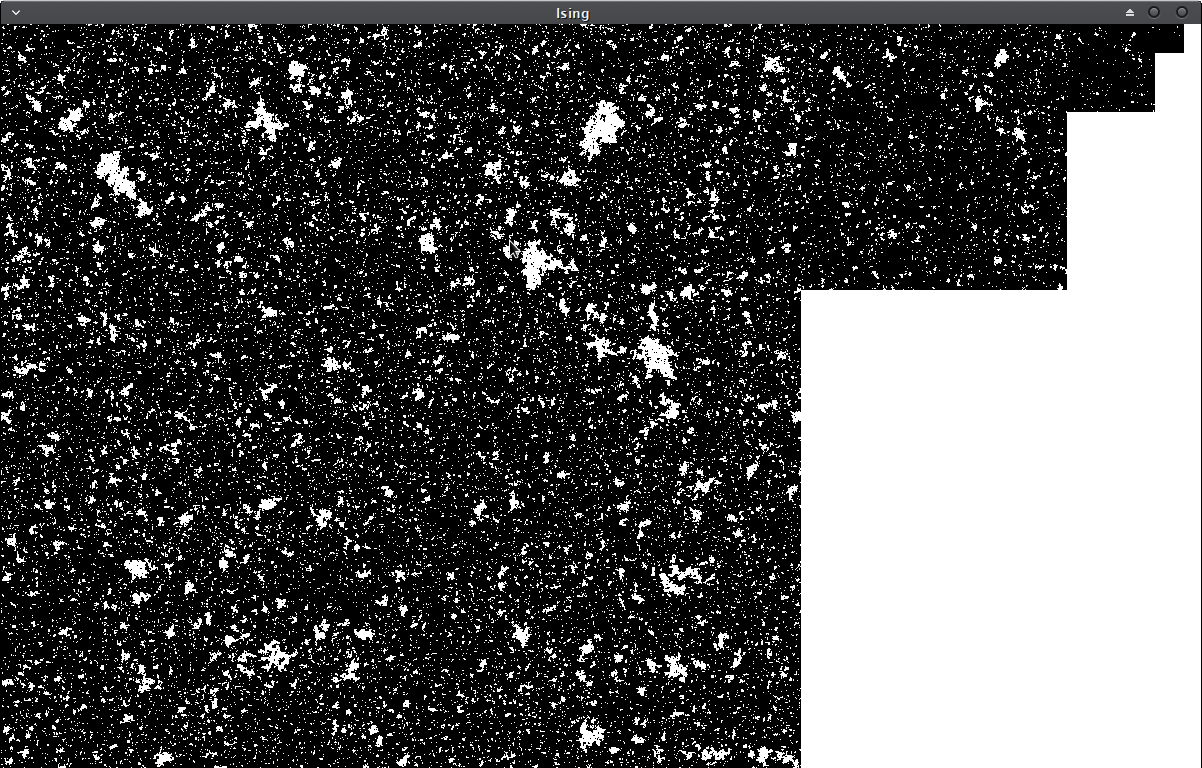
\includegraphics[width=1\linewidth]{TD3/decim_T_sur_Tc_0.98.png}\\

Bien sûr, les configurations de plus grande échelle obtenues sont plus petites, mais ce qui nous intéresse est : \emph{à quoi ressemblent-elles ?} Dans le cas ci-dessus, on remarque que l'on tend vers une configuration uniformément magnétisée, les fluctuations disparaissant à grande échelle. Si l'on devrait décrire cette configuration de grande échelle en terme des paramètres initiaux du modèle $J$ et $T$, on dirait que l'on tend à grande échelle vers $T/J\to 0$ (température nulle).\\

On dit qu'à chaque d'étape de changement d'échelle, c'est tout comme si on avait encore un modèle d'Ising, mais avec $J$ et $T$ \emph{renormalisés}. Les techniques dites "de renormalisation" ont précisemment pour objectif de voir vers quels valeurs de paramètres tend-t-on lorsque l'on tend à grande échelle, avec des méthodes numériques ou analytiques. Il s'agit d'une idée centrale dans l'étude moderne des transitions de phases, et d'une grande puissance.\\

Nous allons nous contenter ici de regarder à quoi ressemble le système "dézoomé" pour différentes températures. Le code suivant est une ébauche d'une fonction prennant un objet \inline{Réseau} carré, et retournant un objet \inline{Réseau} de taille inférieure, résulat de la procédure de décimation expliquée ci-dessus.

\begin{minted}[fontsize=\footnotesize,mathescape=true]{c++}
Réseau decimate (const Réseau& S) {

  // Création d'un sur-réseau de taille $N\times N$ lorsque le réseau initial est de taille $3N\times 3N$
  Réseau S_decim (r.nx / 3, r.ny / 3);

  // On parcours les sites dans le sur-réseau
  for (int x_decim = 0; x_decim < S_decim.nx; x_decim++) {
    for (int y_decim = 0; y_decim < S_decim.ny; y_decim++) {
      Site s = S_decim.site_xy(x_decim,y_decim);

      // Calcul de la somme des spins sur la plaquette de $3 \times 3$ associée à notre "sur-site"
      int8_t sum = 0;
      for (int dx = -1; dx <= +1; dx++) {
        for (int dy = -1; dy <= +1; dy++) {
          sum += S[S.site_xy(
            3 * x_decim + 1 + dx,
            3 * y_decim + 1 + dy
          )];
        }
      }

      S_decim[s] = /*...*/;
    }
  }
  return S_decim;
}
\end{minted}

Complétez le code et testez si il produit bien le résultat attendu. Explorez ensuite à quoi ressemble le système "dézoomé" pour différentes températures. Qu'avons-nous au point critique ?

\begin{correction}
Pour déterminer la valeur de notre sur-site, il suffit de faire la somme des sites de la plaquette. Si les sites \emph{down} sont majoritaires, la somme sera négative, et on attribue $-1$. Sinon, la somme est positive, et on attribue $+1$. Comme le nombre de sites est impair, on ne peut jamais tomber sur une somme valant $0$.

\begin{minted}[fontsize=\footnotesize]{c++}
S_decim[s] = (sum > 0) ? 1 : -1;
\end{minted}

On a déjà vu que pour $T<T_\text{c}$ ($T=0.98\,T_\text{c}$ ci-dessus), le système ressemble à un système de température nulle à grande échelle (système décimé uniformément noir ou blanc, complètement magnétisé et sans fluctuations thermiques).\\

Pour $T>T_\text{c}$, au contraire, le système semble de plus en plus désorganisé à grande échelle :\\
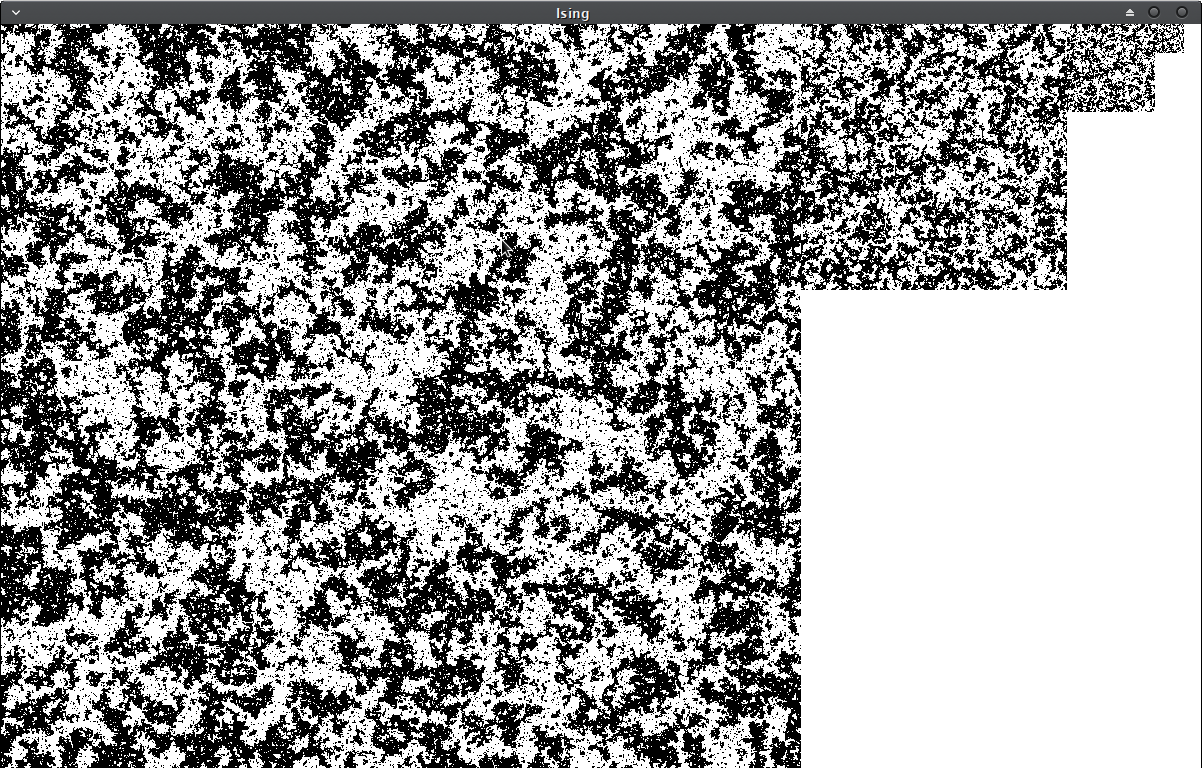
\includegraphics[width=1\linewidth]{TD3/decim_T_sur_Tc_1.1.png}\\
(ici pour $T=1.1\,T_\text{c}$). Il n'y a plus aucune magnétisation dans le système décimé, même locale (pas de zones organisées). Cela ressemble donc à un système de température infinie (ou sans interactions).\\

Enfin, pour $T = T_\text{c}$, on obtient par exemple ceci :\\
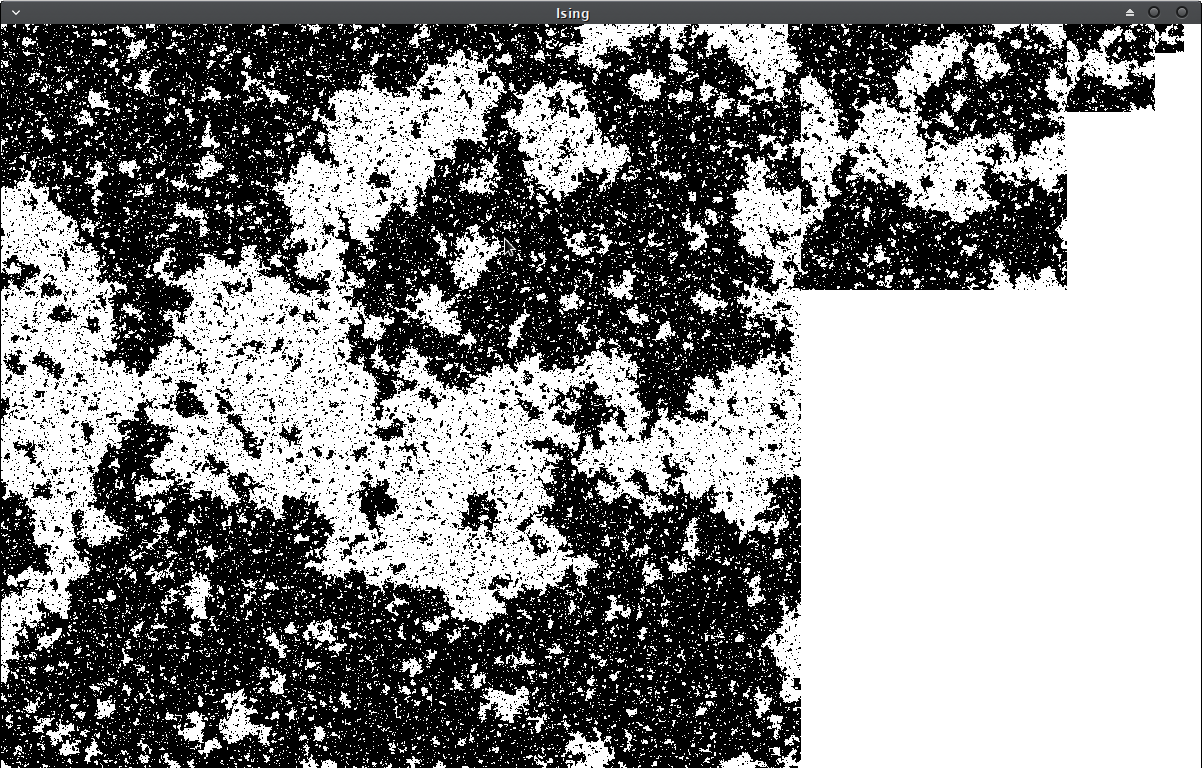
\includegraphics[width=1\linewidth]{TD3/decim_T_sur_Tc_1.00.png}\\
On remarque que le structure spatiale du système ne semble pas vraiment changer avec la décimation : le système décimé pourrait tout à faire être un petit bout du système initial, ce qui n'était pas le cas pour $T = T_\text{c}$. Le système semble alors auto-similaire, "fractal", on a \emph{invariance d'échelle}. Cela ressemble donc à un système à $T = T_\text{c}$. Autrement dit, \emph{le point critique est un point fixe de la procédure de renormalisation par changement d'échelle} :

\begin{center}
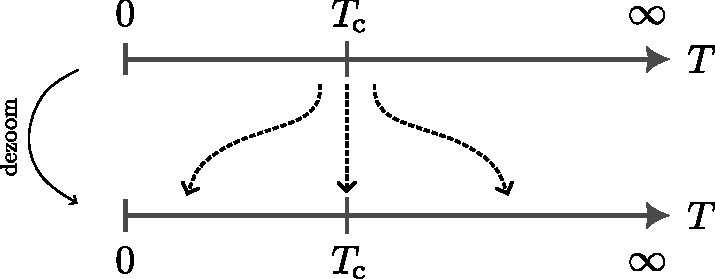
\includegraphics[width=0.5\linewidth]{TD3/renorm.pdf}
\end{center}

\end{correction}

%-----------------------------------

\section{[Bonus] Que coûtent l'abstraction et la compilation séparée ?}

Nous avons mentionné l'utilisation des options \inline{-Ofast -flto} pour obtenir de bonnes performances. Expliquons pourquoi.\\

La première option, que l'on utilise à la compilation (l'étape \texttt{.cpp} $\to$ \texttt{.o}) et qui fait partie de la série d'options \inline{-O0}, \inline{-O1}, \inline{-O2}, \inline{-O3}, \inline{-Ofast}, indique au compilateur d'effectuer toutes les optimisations qu'il peut pour accélérer l'exécution du programme (élimination des valeurs temporaires et des copies, ré-ordonnancement du code, déroulage des boucles, et bien d'autres optimisations encore). L'option \inline{-O0} désactive toute optimisation (parfois pratique pour le déboguage), et \inline{-O3}/\inline{-Ofast} activent toutes les optimsations. La différence entre \inline{-O3} et \inline{-Ofast} est que le deuxième privilégie la vitesse à tout prix, au détriment de la taille de l'exécutable, ce qui n'est pas toujours une bonne idée.\\

Testez votre programme, avec une durée de simulation finie de l'ordre de $10\,\mathrm{s}$, en compilant avec \inline{-O1}, \inline{-O3} et \inline{-Ofast}, et sans \inline{-flto}. Utilisez la commande unix \texttt{time [programme]} pour mesurer le temps d'exécution. Ajoutez ensuite \inline{-Ofast -flto} à la compilation et à l'édition de liens (l'étape \{\texttt{.o}\} $\to$ exécutable). Voyez-vous une grosse différence ?\\

L'option \inline{-flto} est là pour régler un problème majeur qui vient avec l'utilisation de plusieurs fichiers \texttt{.cpp}, et donc \texttt{.o} différents. En effet, lors de la compilation de \texttt{ising.cpp} en \texttt{ising.o}, le compilateur n'a aucune idée de ce qui se passe dans \texttt{reseau.cpp}. Il sait juste que les fonctions de \texttt{reseau.h} ont été déclarées. Il n'est donc pas possible d'effectuer des optimisations concernant l'appel de fonctions entre \texttt{ising.cpp} et \texttt{reseau.cpp}, par exemple l'élimination de copie ou même l'élimination des appels de fonction en copiant la fonction à l'endroit où elle est utilisée (\emph{inlining}). On perd donc une grosse opportunité d'optimisation, surtout pour ce TD où les fonctions de \inline{Réseau} méritent d'être inlinées. L'option \inline{-flto}, pour \emph{link time optimization}, rajoute un deuxième round d'optimisations au moment où l'édition de liens entre les \texttt{.o} est effectuée. À ce moment là, et à ce moment là seulement, le compilateur a une vue globale de tout le code, et peut donc effectuer toutes les optimisations.\\

Pour vérifier que l'on ne perd pas de performance par rapport à un code avec beaucoup moins d'abstraction, écrit "à la C" (impératif) et dans un seul fichier, comparez avec le programme \filename{TD3/ising\_monolithique.cpp}, où vous adapterez la taille du système et le nombre d'itérations pour que cela corresponde à votre programme. Voyez-vous une différence de performance ?

\begin{correction}
Le tableau suivant montre le temps d'exécution pour $2\cdot 10^8$ pas de l'algorithme, pour un réseau carré de $200 \times 200$, sur un ordinateur portable des années 2010 de performances moyennes, et sur Linux.
\begin{table}[H]
\hspace*{-0.45cm}%
\begin{tabular}{cccc|cc}
\hline
\multicolumn{4}{c|}{\textit{\textbf{Code orienté objet avec fichiers séparés}}}                                                                                 & \multicolumn{2}{c}{\textit{\textbf{Code impératif monolithique}}}      \\
\multicolumn{1}{c|}{gcc \texttt{-O1}} & \multicolumn{1}{c|}{gcc \texttt{-Ofast}} & \multicolumn{1}{c|}{gcc \texttt{-Ofast -flto}} & clang \texttt{-Ofast -flto} & \multicolumn{1}{c|}{gcc \texttt{-Ofast}} & clang \texttt{-Ofast -flto} \\ \hline
\multicolumn{1}{c|}{32.5 s}           & \multicolumn{1}{c|}{18.2 s}              & \multicolumn{1}{c|}{\textbf{8.2 s}}            & 8.9 s                       & \multicolumn{1}{c|}{\textbf{7.7 s}}      & 8.0 s                       \\ \hline
\end{tabular}
\end{table}
On remarque les performances catastrophiques du programme lorsqu'il manque l'optimisation au niveau de la compilation \texttt{-Ofast/-O3} et/ou l'optimisation au niveau de l'édition de liens \texttt{-flto}.\\

On remarque aussi que avec \texttt{-Ofast -flto}, le temps d'exécution est très similaire à celui du programme monolithique impératif. On peut donc conclure que l'ajout de couches d'abstractions et la séparation en multiples fichiers, lorsque le code est conçu correctement, n'apporte pas de dégradation de performances significatives. Il en serait tout autre avec un langage interprété comme le Python.\\

Enfin, la différence entre les compilateurs gcc et clang est faible lorsque toutes les optimisations sont activés.
\end{correction}

\end{document}
